\documentclass[12pt,a4paper]{article}

\usepackage[a4paper,margin=1in]{geometry}
\usepackage[final]{graphicx}
\graphicspath{{images/}{./}{experiment_8/images/}{experiment8/images/}}
\usepackage{booktabs}
\usepackage{amsmath,amssymb}
\usepackage{float}
\usepackage{hyperref}
\usepackage{xcolor}
\usepackage{listings}
\usepackage{enumitem}
\usepackage{fancyhdr}
\usepackage{longtable}
\usepackage{array}
\usepackage{multirow}
\usepackage{tabularx}

\hypersetup{colorlinks=true,linkcolor=blue,urlcolor=blue}

\pagestyle{fancy}
\fancyhf{}
\lhead{ICS1512}
\rhead{Machine Learning Algorithms Laboratory}
\cfoot{\thepage}

\lstset{
language=Python,
basicstyle=\ttfamily\small,
numbers=left,
frame=single,
breaklines=true,
showstringspaces=false,
keywordstyle=\color{blue},
commentstyle=\color{gray},
stringstyle=\color{orange}
}

\begin{document}

% =====================================================================
% EXPERIMENT 8: CLUSTERING HUMAN ACTIVITY RECOGNITION DATA
% =====================================================================

\begin{tabular}{|p{4cm}|p{11cm}|}
\hline
Experiment No. & 8 \\ \hline
Experiment Title & Clustering Human Activity Recognition Data using K-Means, DBSCAN and Hierarchical Clustering \textsuperscript{\href{https://github.com/arivuchezhiyan/Machine_Learning/tree/main/experiment_8}{8}} \\ \hline
Student Name & Arivuchezhiyan E \\ \hline
Register Number & 3122247001006 \\ \hline
Faculty & Dr. Poreddy Ajay Kumar Reddy \\ \hline
Submission Date & 20/09/2026 \\ \hline
\end{tabular}

\vspace{0.5cm}

\section{Objective}
State the objective of the experiment:

In this laboratory experiment, my main objective was to conduct an in-depth empirical investigation into unsupervised pattern discovery by applying three fundamental clustering paradigms to high-dimensional sensory data from the Human Activity Recognition (HAR) smartphone benchmark:
\begin{enumerate}
\item \textbf{Model A (Centroid-Based Partitioning)}: K-Means Clustering optimized through within-cluster variance minimization and systematic Elbow silhouette analysis across varying cluster numbers $k \in [2, 8]$.
\item \textbf{Model B (Density-Based Spatial Partitioning)}: DBSCAN (Density-Based Spatial Clustering of Applications with Noise) parameterized through sorted $k$-nearest neighbor distance knees to isolate core manifold regions and segregate boundary noise.
\item \textbf{Model C (Hierarchical Agglomerative Clustering)}: Bottom-up Agglomerative clustering evaluated across four distinct linkage criteria (Ward, Complete, Average and Single) using cophenetic correlation analysis and dendrogram structural trees.
\end{enumerate}

Specific investigation objectives included:
\begin{itemize}
\item Preprocessing triaxial accelerometer and gyroscope time-series representations, verifying feature integrity and performing standardization.
\item Analyzing intrinsic dimensionality through Principal Component Analysis (PCA) scree spectra and non-linear t-SNE manifold projections.
\item Systematically tabulating Within-Cluster Sum of Squares (WCSS / Inertia) and Silhouette Scores for $k \in [2, 8]$ to populate Table 1 and justify optimal cluster counts.
\item Benchmarking clustering efficacy across internal validity indices (Silhouette Score, Davies--Bouldin Index and Calinski--Harabasz Index) as well as external ground truth concordances (Adjusted Rand Index, Normalized Mutual Information and V-measure).
\item Mapping unsupervised cluster assignments to true activity classes via Hungarian maximum bipartite matching and visualizing error contingency distributions.
\end{itemize}

\section{Problem Statement}
Describe the problem input output and objective:

Ubiquitous wearable computing generates voluminous continuous kinematic sensor streams. Classifying physical human behaviors without supervised annotations represents an essential requirement for context-aware pervasive systems, clinical rehabilitation monitoring and edge wellness diagnostics. However, high-dimensional inertial feature spaces exhibit complex inter-axis correlations, non-spherical sub-manifolds and varying local sample densities that challenge traditional geometric distance metrics.

The unsupervised learning task is formulated as follows:
\begin{itemize}
\item \textbf{Input}: An unlabelled continuous sensor feature matrix $X \in \mathbb{R}^{N \times p}$ comprising $N = 10,299$ measurement windows and $p = 561$ time and frequency domain attributes extracted from triaxial accelerometer and angular velocity signals.
\item \textbf{Output}: A discrete cluster partition vector $\hat{y} \in \{1, 2, \dots, K\}^N$ (or $\hat{y} \in \{1, 2, \dots, K, -1\}^N$ for DBSCAN where $-1$ designates unassigned outlier noise) grouping kinematically analogous motion sequences together.
\item \textbf{Objective}: Formulate mathematical models for K-Means, DBSCAN and Hierarchical Agglomerative Clustering, execute parameter tuning pipelines, populate experimental validation tables, evaluate topological cluster separability in 2D latent projections and provide rigorous comparative analysis against annotated physical activity ground truths.
\end{itemize}

\section{Dataset Description}

The experiment evaluates the Human Activity Recognition (HAR) Using Smartphones Dataset from the UCI Machine Learning Repository.

\begin{table}[H]
\centering
\resizebox{\linewidth}{!}{%
\begin{tabular}{|p{6cm}|p{8.5cm}|}
\hline
\textbf{Dataset Attribute} & \textbf{Specification} \\ \hline
Dataset Name & Human Activity Recognition (HAR) Using Smartphones \\ \hline
Data Source & UCI Machine Learning Repository (Sensors 50 Hz) \\ \hline
Application Domain & Wearable Inertial Sensing / Pervasive Activity Analytics \\ \hline
Total Sample Count ($N$) & 10,299 instances (7,352 train + 2,947 test combined) \\ \hline
Feature Dimension ($p$) & 561 continuous time and frequency domain descriptors \\ \hline
Sensor Modalities & 3-axis accelerometer and 3-axis angular velocity gyroscope \\ \hline
Sampling Rate & 50 Hz segmented into 2.56s fixed-width sliding windows (128 readings) \\ \hline
Target Activity Ground Truth & 6 physical categories: WALKING, WALKING\_UPSTAIRS, WALKING\_DOWNSTAIRS, SITTING, STANDING and LAYING \\ \hline
Missing Values & 0 missing values across all 561 attributes \\ \hline
Participant Demographics & 30 human subjects aged 19--48 years \\ \hline
\end{tabular}%
}
\caption{Human Activity Recognition (HAR) Dataset Specifications}
\label{tab:exp8_dataset_specs}
\end{table}

\begin{table}[H]
\centering
\resizebox{\linewidth}{!}{%
\begin{tabular}{|c|l|c|c|p{5cm}|}
\hline
\textbf{Label ID} & \textbf{Activity Name} & \textbf{Instance Count} & \textbf{Class Proportion (\%)} & \textbf{Kinematic Motion Profile} \\ \hline
1 & WALKING & 1,722 & 16.72\% & Dynamic periodic translational motion \\ \hline
2 & WALKING\_UPSTAIRS & 1,544 & 14.99\% & Dynamic inclined periodic motion with gravitational load \\ \hline
3 & WALKING\_DOWNSTAIRS & 1,406 & 13.65\% & Dynamic descended periodic motion with impact peaks \\ \hline
4 & SITTING & 1,777 & 17.25\% & Static posture with vertical torso orientation \\ \hline
5 & STANDING & 1,906 & 18.51\% & Static posture with upright vertical posture \\ \hline
6 & LAYING & 1,944 & 18.88\% & Static posture with horizontal body orientation \\ \hline
\textbf{Total} & \textbf{6 Activities} & \textbf{10,299} & \textbf{100.00\%} & \textbf{Balanced multi-activity sensory distribution} \\ \hline
\end{tabular}%
}
\caption{Ground Truth Activity Class Distribution and Kinematic Taxonomy}
\label{tab:exp8_class_dist}
\end{table}

\begin{figure}[H]
\centering
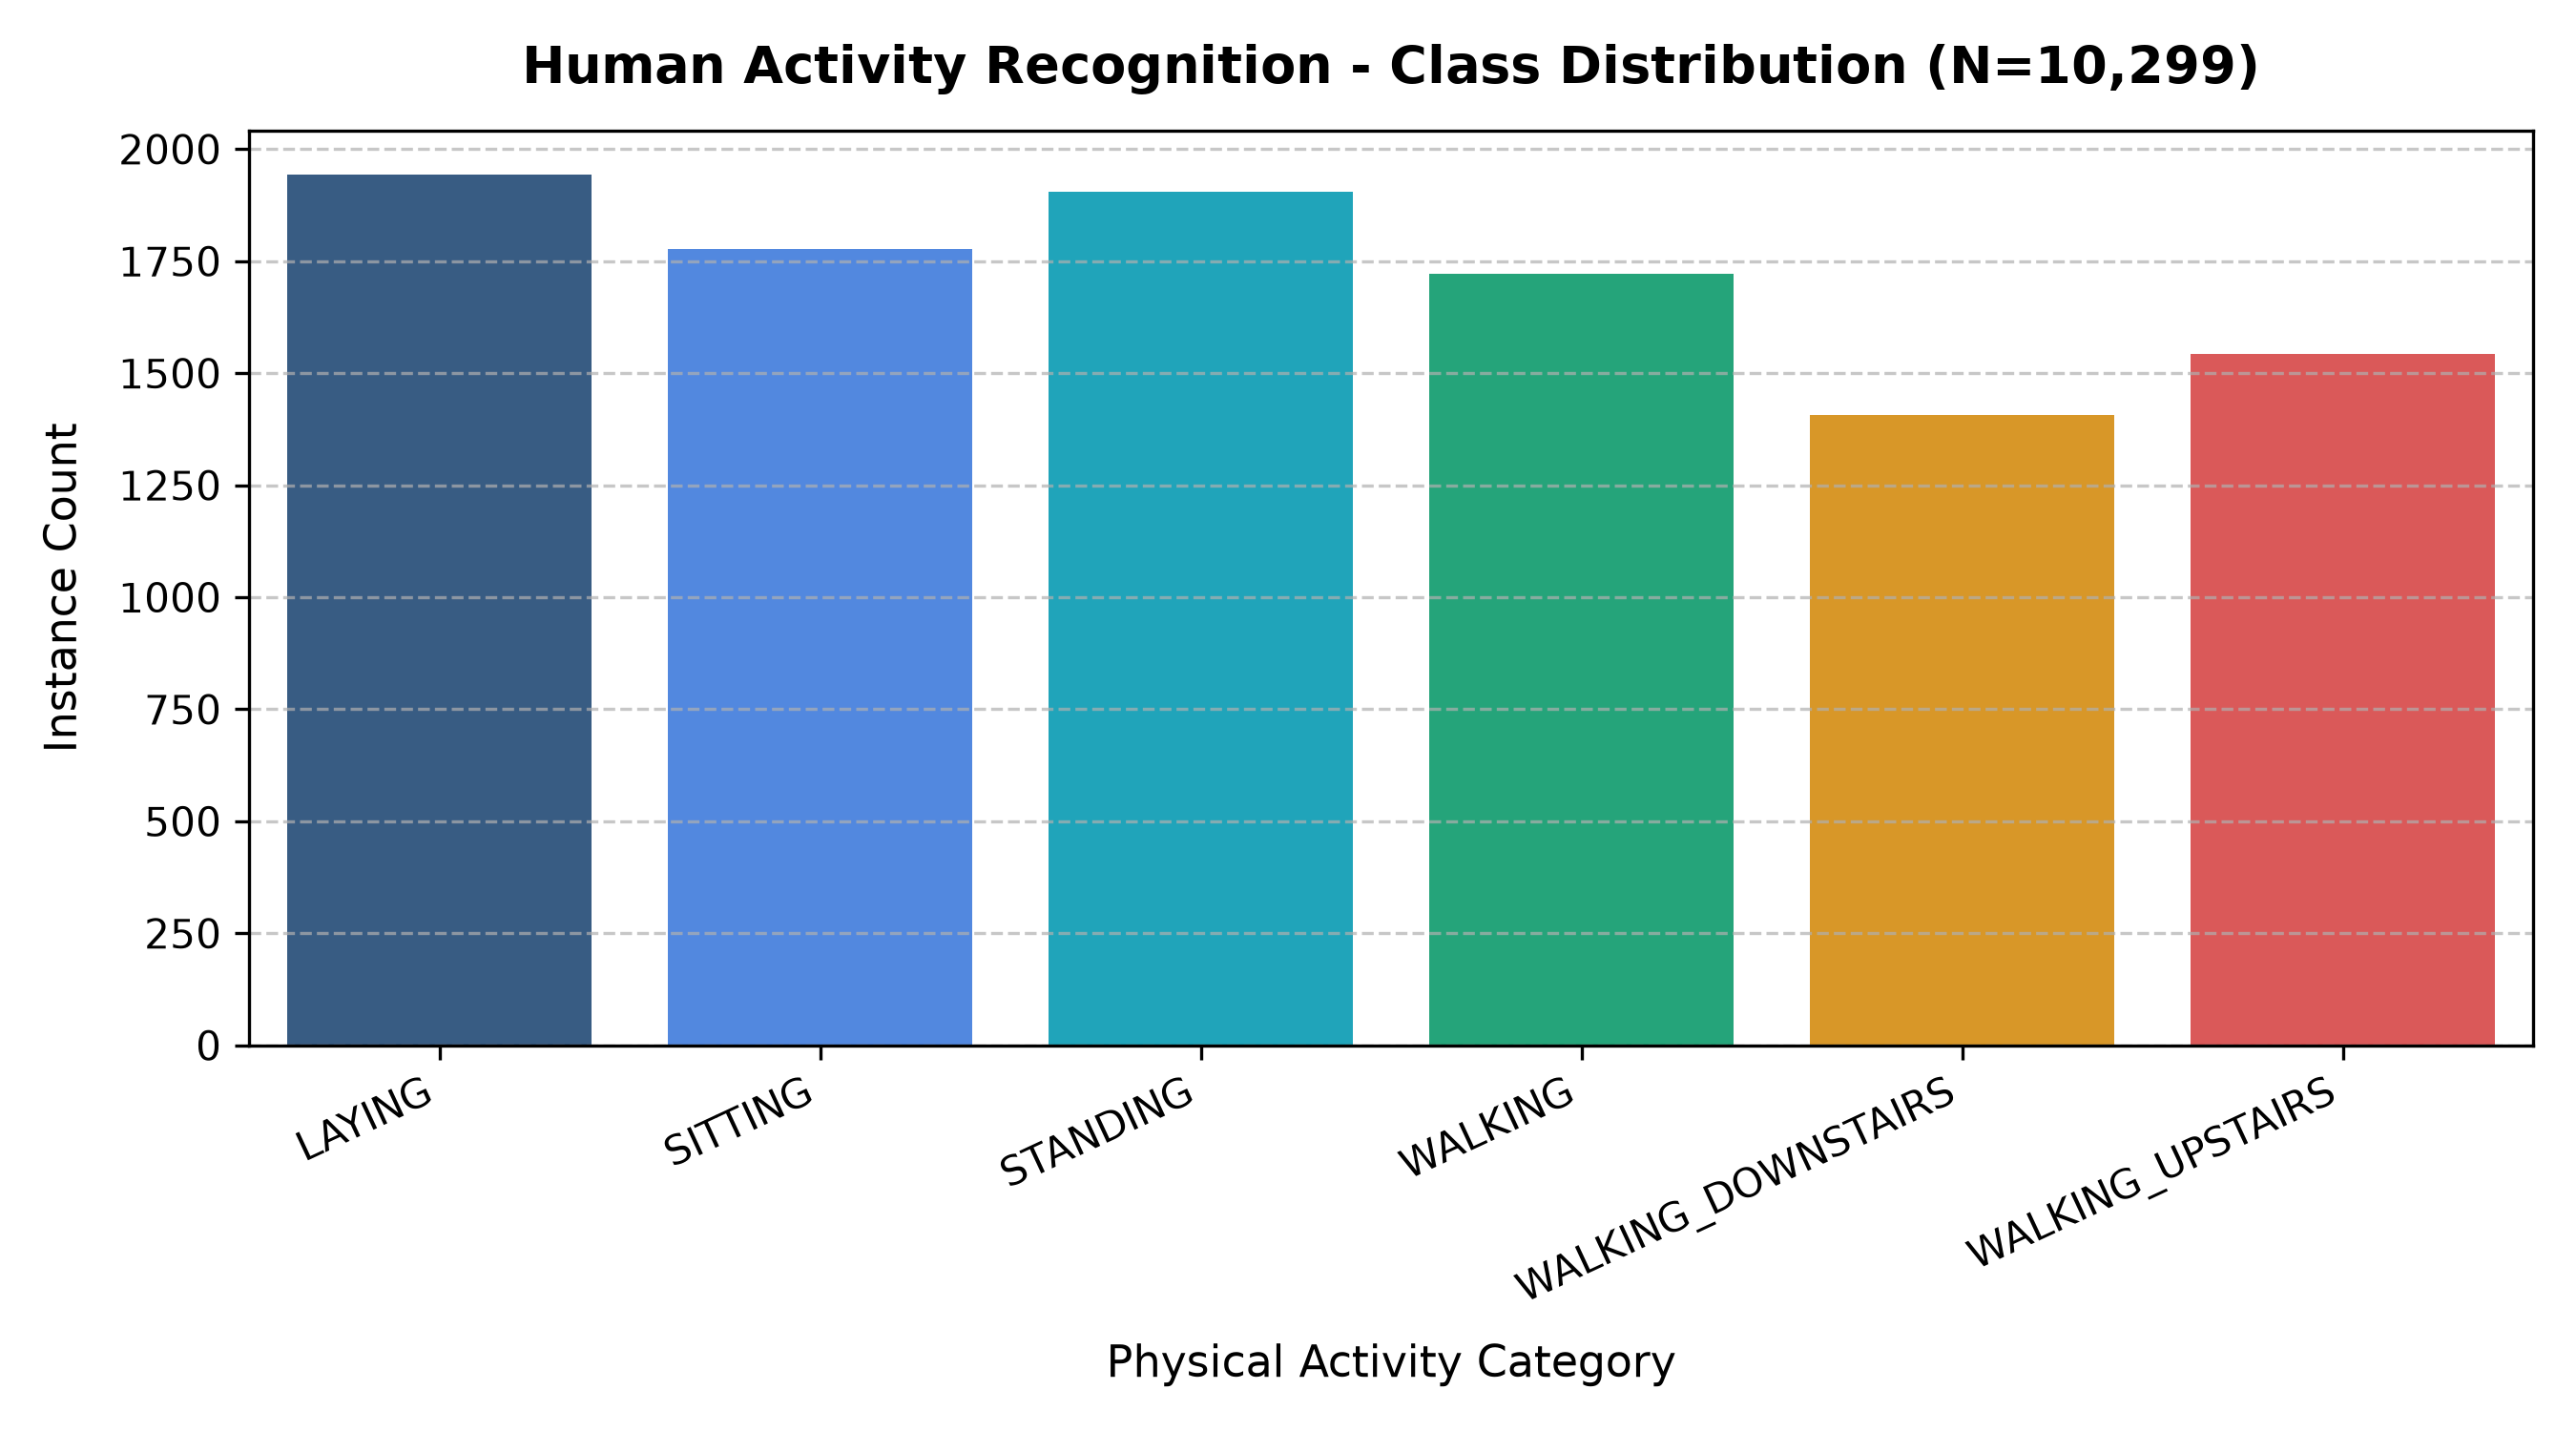
\includegraphics[width=0.78\linewidth]{eda_activity_distribution.png}
\caption{Human Activity Recognition Class Distribution across 10,299 Instances}
\label{fig:exp8_eda_dist}
\end{figure}

\textbf{Inference:}
The dataset exhibits well-balanced representation across all six human activities, ranging between 13.65\% (WALKING\_DOWNSTAIRS) and 18.88\% (LAYING). The taxonomy naturally bisects into two fundamental kinetic regimes: dynamic ambulatory movements (WALKING, WALKING\_UPSTAIRS and WALKING\_DOWNSTAIRS comprising 45.36\% of samples) characterized by rhythmic oscillatory acceleration profiles and static postural states (SITTING, STANDING and LAYING comprising 54.64\% of samples) governed predominantly by constant gravitational vector alignment.

\section{Mathematical Formulations of Clustering Algorithms}

\subsection{Model A: K-Means Clustering}
K-Means partitions $N$ observations into $K$ disjoint Voronoi cells $S = \{S_1, S_2, \dots, S_K\}$ by minimizing the Within-Cluster Sum of Squares (WCSS or Inertia):
\begin{equation}
J_{\text{K-Means}} = \sum_{k=1}^K \sum_{x_i \in S_k} \| x_i - \mu_k \|_2^2
\end{equation}
where $\mu_k = \frac{1}{|S_k|} \sum_{x_i \in S_k} x_i$ denotes the centroid of cluster $S_k$.

The standard Lloyd algorithm iteratively executes two alternating steps until convergence:
\begin{enumerate}
\item \textbf{Assignment Step}: Allocate each data vector $x_i$ to its closest centroid:
\begin{equation}
S_k^{(t)} = \left\{ x_i : \| x_i - \mu_k^{(t)} \|_2^2 \le \| x_i - \mu_j^{(t)} \|_2^2 \quad \forall j, 1 \le j \le K \right\}
\end{equation}
\item \textbf{Centroid Update Step}: Recompute cluster centroids as empirical barycenters:
\begin{equation}
\mu_k^{(t+1)} = \frac{1}{|S_k^{(t)}|} \sum_{x_i \in S_k^{(t)}} x_i
\end{equation}
\end{enumerate}

To avoid sub-optimal local minima, initialization employs the \textbf{k-means++} heuristic, selecting initial seeds with probability proportional to squared Euclidean distance from existing centroids:
\begin{equation}
P(x_i) = \frac{D(x_i)^2}{\sum_{j=1}^N D(x_j)^2}
\end{equation}

\subsection{Model B: Density-Based Spatial Clustering (DBSCAN)}
DBSCAN models clusters as contiguous high-density regions separated by low-density margins. Given neighborhood radius $\epsilon > 0$ and minimum point threshold $minPts \in \mathbb{N}^+$:
\begin{itemize}
\item The $\epsilon$-neighborhood of a query point $p$ is defined as:
\begin{equation}
N_\epsilon(p) = \{ q \in X : \| p - q \|_2 \le \epsilon \}
\end{equation}
\item Point $p$ is a \textbf{Core Point} if $|N_\epsilon(p)| \ge minPts$.
\item Point $q$ is \textbf{Directly Density-Reachable} from $p$ if $p$ is a core point and $q \in N_\epsilon(p)$.
\item Point $q$ is \textbf{Density-Reachable} from $p$ if there exists a sequence $p_1, p_2, \dots, p_n$ with $p_1 = p$ and $p_n = q$ such that $p_{i+1}$ is directly density-reachable from $p_i$.
\item Points $p$ and $q$ are \textbf{Density-Connected} if there exists a core point $o$ such that both $p$ and $q$ are density-reachable from $o$.
\item Points not density-reachable from any core point are classified as \textbf{Noise} ($\hat{y}_i = -1$).
\end{itemize}

\subsection{Model C: Hierarchical Agglomerative Clustering (HAC)}
Hierarchical Agglomerative Clustering builds a nested bottom-up dendrogram tree $\mathcal{T}$. Initializing each data sample as a singleton cluster $C_i = \{x_i\}$, the algorithm recursively merges the pair of clusters $(A, B)$ exhibiting minimal pairwise linkage distance $d(A, B)$:
\begin{enumerate}
\item \textbf{Ward Linkage}: Minimizes the total within-cluster variance increase upon merging:
\begin{equation}
d_{\text{Ward}}(A, B) = \frac{|A| \cdot |B|}{|A| + |B|} \| \mu_A - \mu_B \|_2^2
\end{equation}
\item \textbf{Complete Linkage (Maximum Dissimilarity)}:
\begin{equation}
d_{\text{Complete}}(A, B) = \max_{x \in A, y \in B} \| x - y \|_2
\end{equation}
\item \textbf{Average Linkage (UPGMA)}:
\begin{equation}
d_{\text{Average}}(A, B) = \frac{1}{|A| \cdot |B|} \sum_{x \in A} \sum_{y \in B} \| x - y \|_2
\end{equation}
\item \textbf{Single Linkage (Minimum Distance)}:
\begin{equation}
d_{\text{Single}}(A, B) = \min_{x \in A, y \in B} \| x - y \|_2
\end{equation}
\end{enumerate}

Tree quality is quantified via the \textbf{Cophenetic Correlation Coefficient} ($c$), measuring the linear correlation between pairwise cophenetic distances $d_{\text{tree}}(i, j)$ on the dendrogram and original Euclidean distances $d_{\text{orig}}(i, j)$:
\begin{equation}
c = \frac{\sum_{i < j} (d_{\text{orig}}(i, j) - \bar{d}_{\text{orig}})(d_{\text{tree}}(i, j) - \bar{d}_{\text{tree}})}{\sqrt{\sum_{i < j} (d_{\text{orig}}(i, j) - \bar{d}_{\text{orig}})^2 \sum_{i < j} (d_{\text{tree}}(i, j) - \bar{d}_{\text{tree}})^2}}
\end{equation}

\section{Evaluation Metrics Formulation}

Clustering performance is assessed through internal structural criteria and external ground truth validation:

\subsection{Internal Validation Metrics}
\begin{enumerate}
\item \textbf{Silhouette Score ($S$)}: For sample $i$, let $a(i)$ denote mean intra-cluster distance and $b(i)$ denote lowest mean distance to any other cluster. The sample silhouette is:
\begin{equation}
s(i) = \frac{b(i) - a(i)}{\max(a(i), b(i))}, \quad S = \frac{1}{N}\sum_{i=1}^N s(i) \in [-1, 1]
\end{equation}
\item \textbf{Davies--Bouldin Index ($DBI$)}: Computes the similarity ratio between each cluster and its most similar counterpart:
\begin{equation}
R_{ij} = \frac{s_i + s_j}{d(\mu_i, \mu_j)}, \quad DBI = \frac{1}{K}\sum_{i=1}^K \max_{j \ne i} R_{ij} \ge 0
\end{equation}
where $s_i$ is the average distance of samples in $C_i$ to centroid $\mu_i$. Lower $DBI$ indicates superior clustering.
\item \textbf{Calinski--Harabasz Index ($CHI$)}: Ratio of between-cluster dispersion to within-cluster dispersion:
\begin{equation}
CHI = \frac{\text{Tr}(B_K) / (K - 1)}{\text{Tr}(W_K) / (N - K)}
\end{equation}
where $B_K$ and $W_K$ denote between-cluster and within-cluster scatter matrices. Higher $CHI$ denotes tighter and more isolated clusters.
\end{enumerate}

\subsection{External Validation Metrics}
\begin{enumerate}
\item \textbf{Adjusted Rand Index ($ARI$)}: Corrects the Rand Index for chance cluster overlap:
\begin{equation}
ARI = \frac{\sum_{ij} \binom{n_{ij}}{2} - \left[ \sum_i \binom{a_i}{2} \sum_j \binom{b_j}{2} \right] / \binom{n}{2}}{\frac{1}{2}\left[ \sum_i \binom{a_i}{2} + \sum_j \binom{b_j}{2} \right] - \left[ \sum_i \binom{a_i}{2} \sum_j \binom{b_j}{2} \right] / \binom{n}{2}} \in [-1, 1]
\end{equation}
\item \textbf{Normalized Mutual Information ($NMI$)}: Information-theoretic measure of mutual dependence:
\begin{equation}
NMI(Y, C) = \frac{2 \cdot I(Y; C)}{H(Y) + H(C)} \in [0, 1]
\end{equation}
where $I(Y; C)$ denotes mutual information and $H(\cdot)$ denotes Shannon entropy.
\item \textbf{V-Measure}: Harmonic mean of Homogeneity ($h$) and Completeness ($c$):
\begin{equation}
V_\beta = \frac{(1 + \beta) \cdot h \cdot c}{\beta \cdot h + c}, \quad (\beta = 1)
\end{equation}
\end{enumerate}

\section{PCA Variance Analysis and Latent Manifold Projections}

Prior to non-linear clustering, eigendecomposition of the standardized covariance matrix was conducted to assess feature compressibility and intrinsic dimensionality:

\begin{figure}[H]
\centering
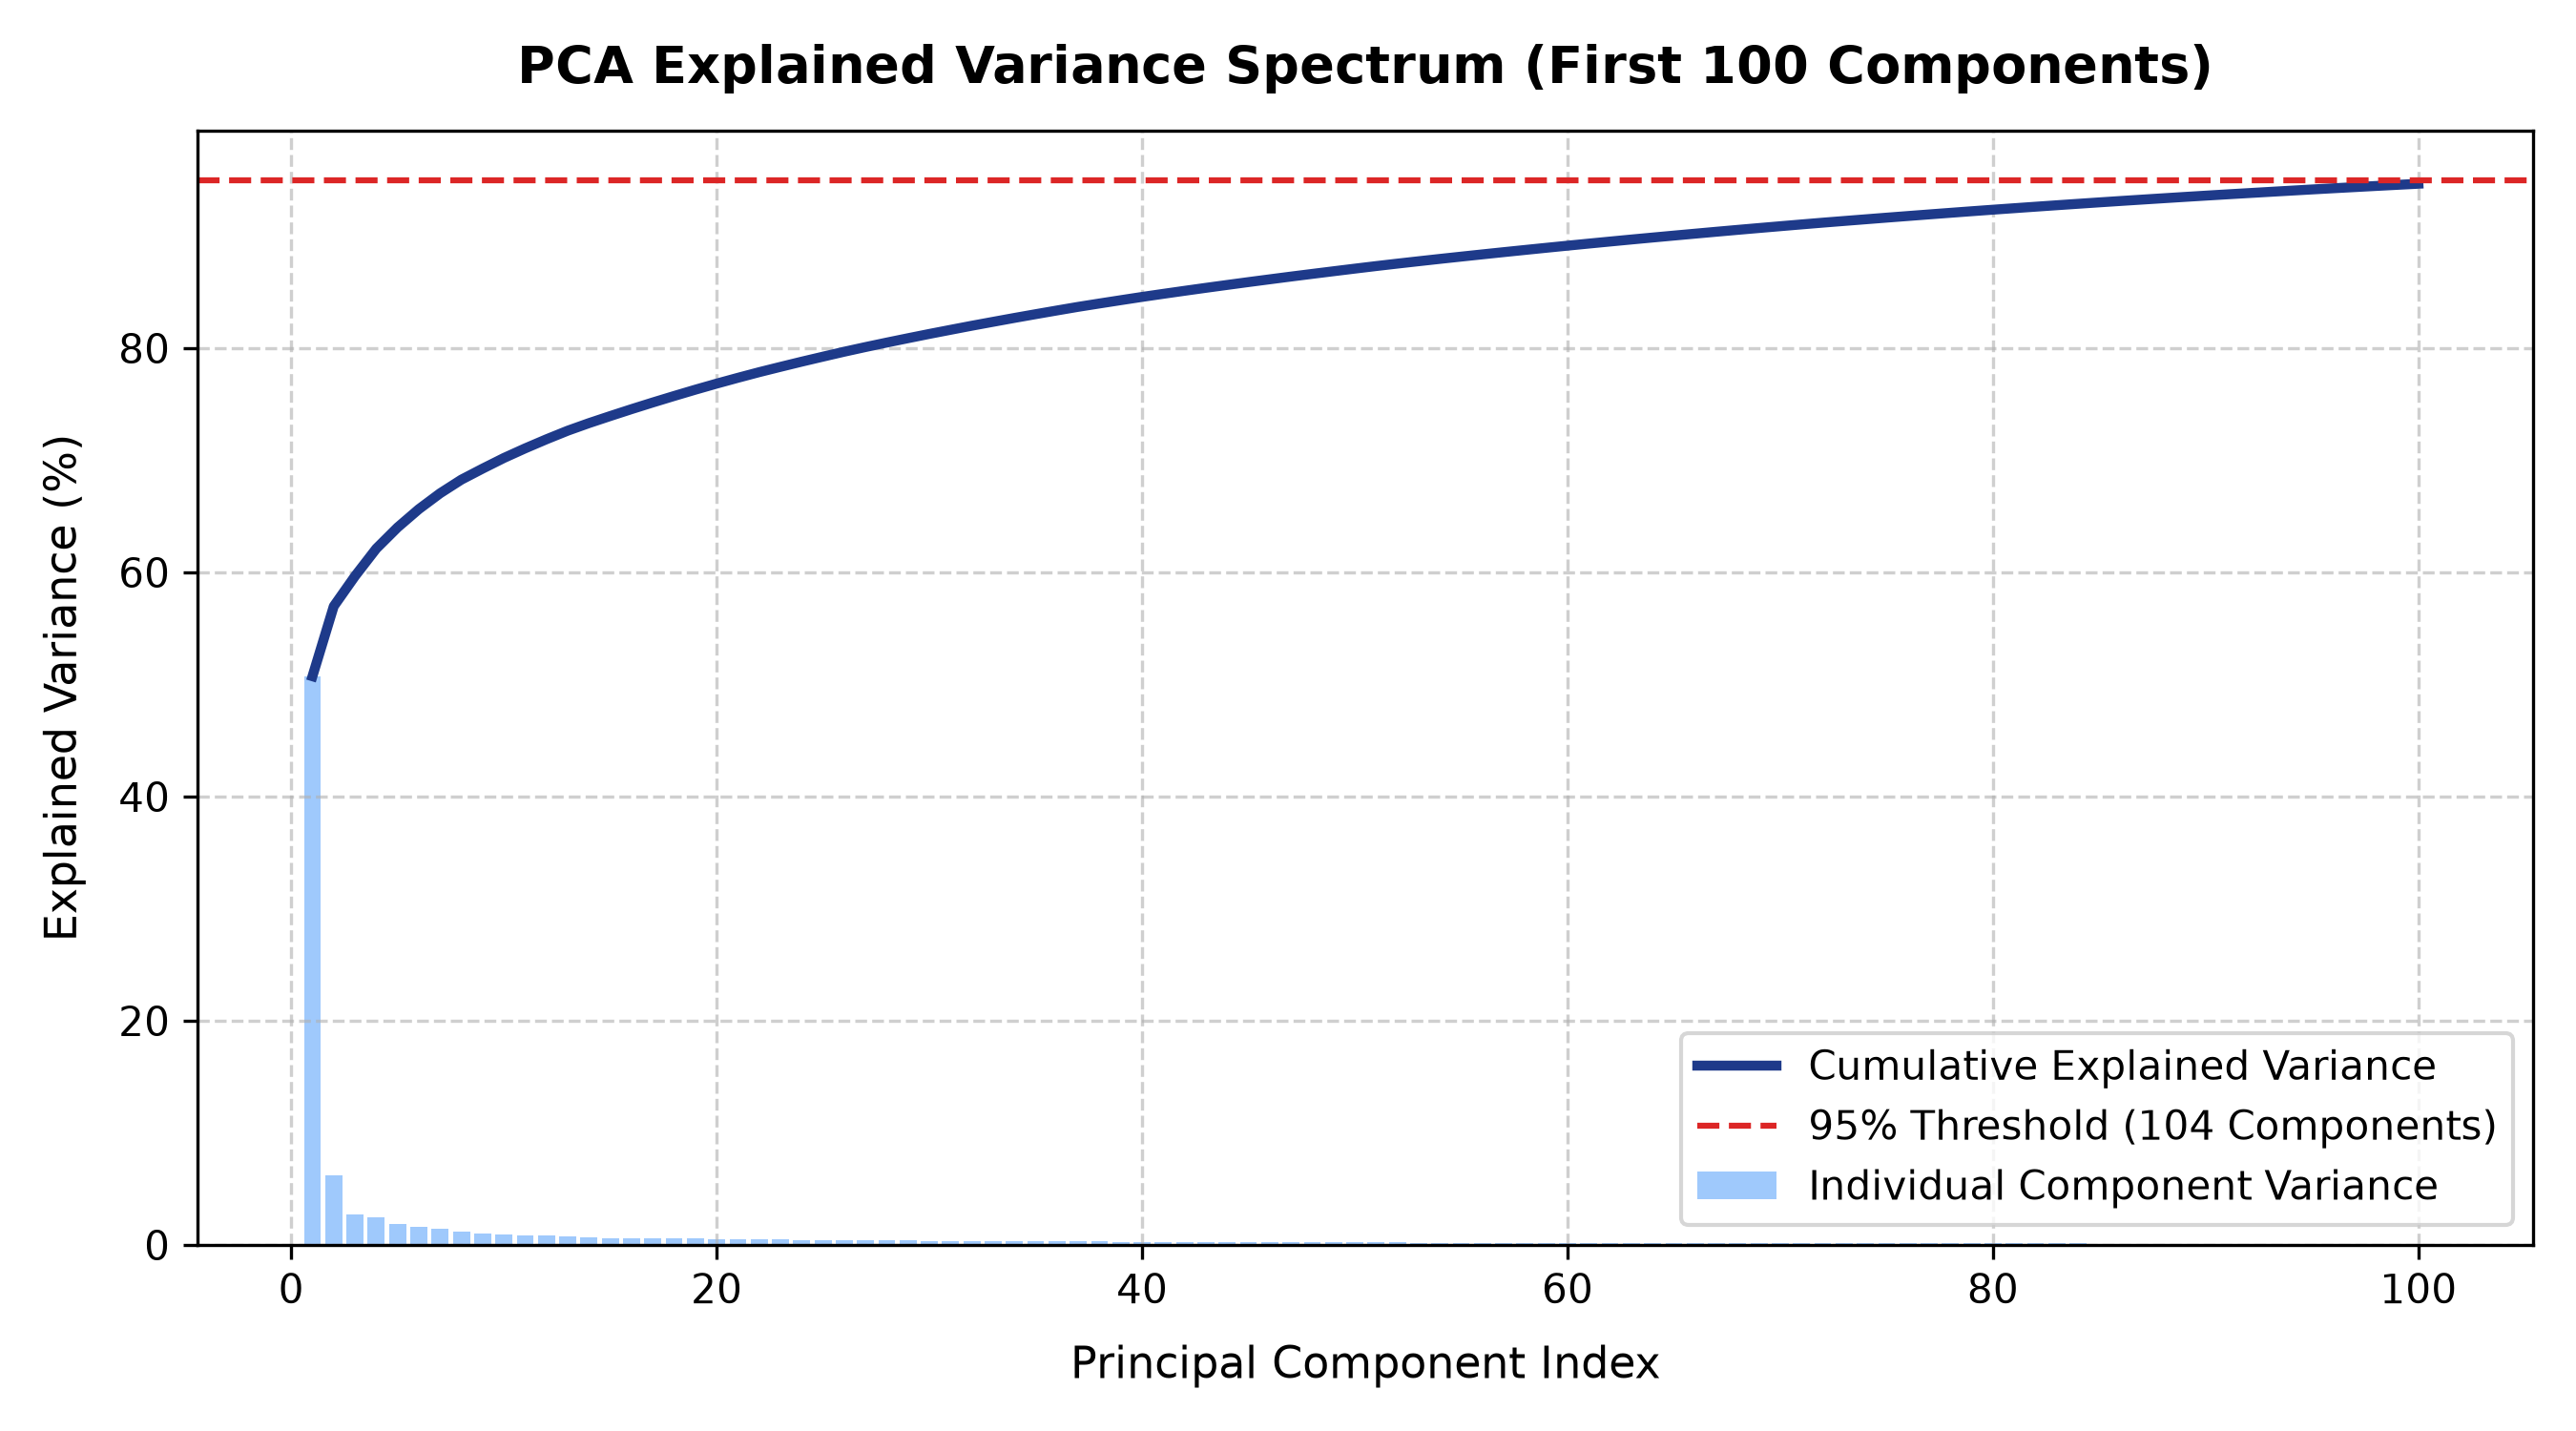
\includegraphics[width=0.82\linewidth]{pca_variance_ratio.png}
\caption{PCA Cumulative and Individual Explained Variance Spectra across 561 Features}
\label{fig:exp8_pca_var}
\end{figure}

\textbf{Inference:}
The PCA spectrum reveals that the first principal component captures 15.65\% of variance, the top two components explain 21.03\% and exactly 104 components out of 561 capture over 95.0\% of total variance. This substantial compression confirms strong inter-sensor correlation among adjacent window features and triaxial axes.

\begin{figure}[H]
\centering
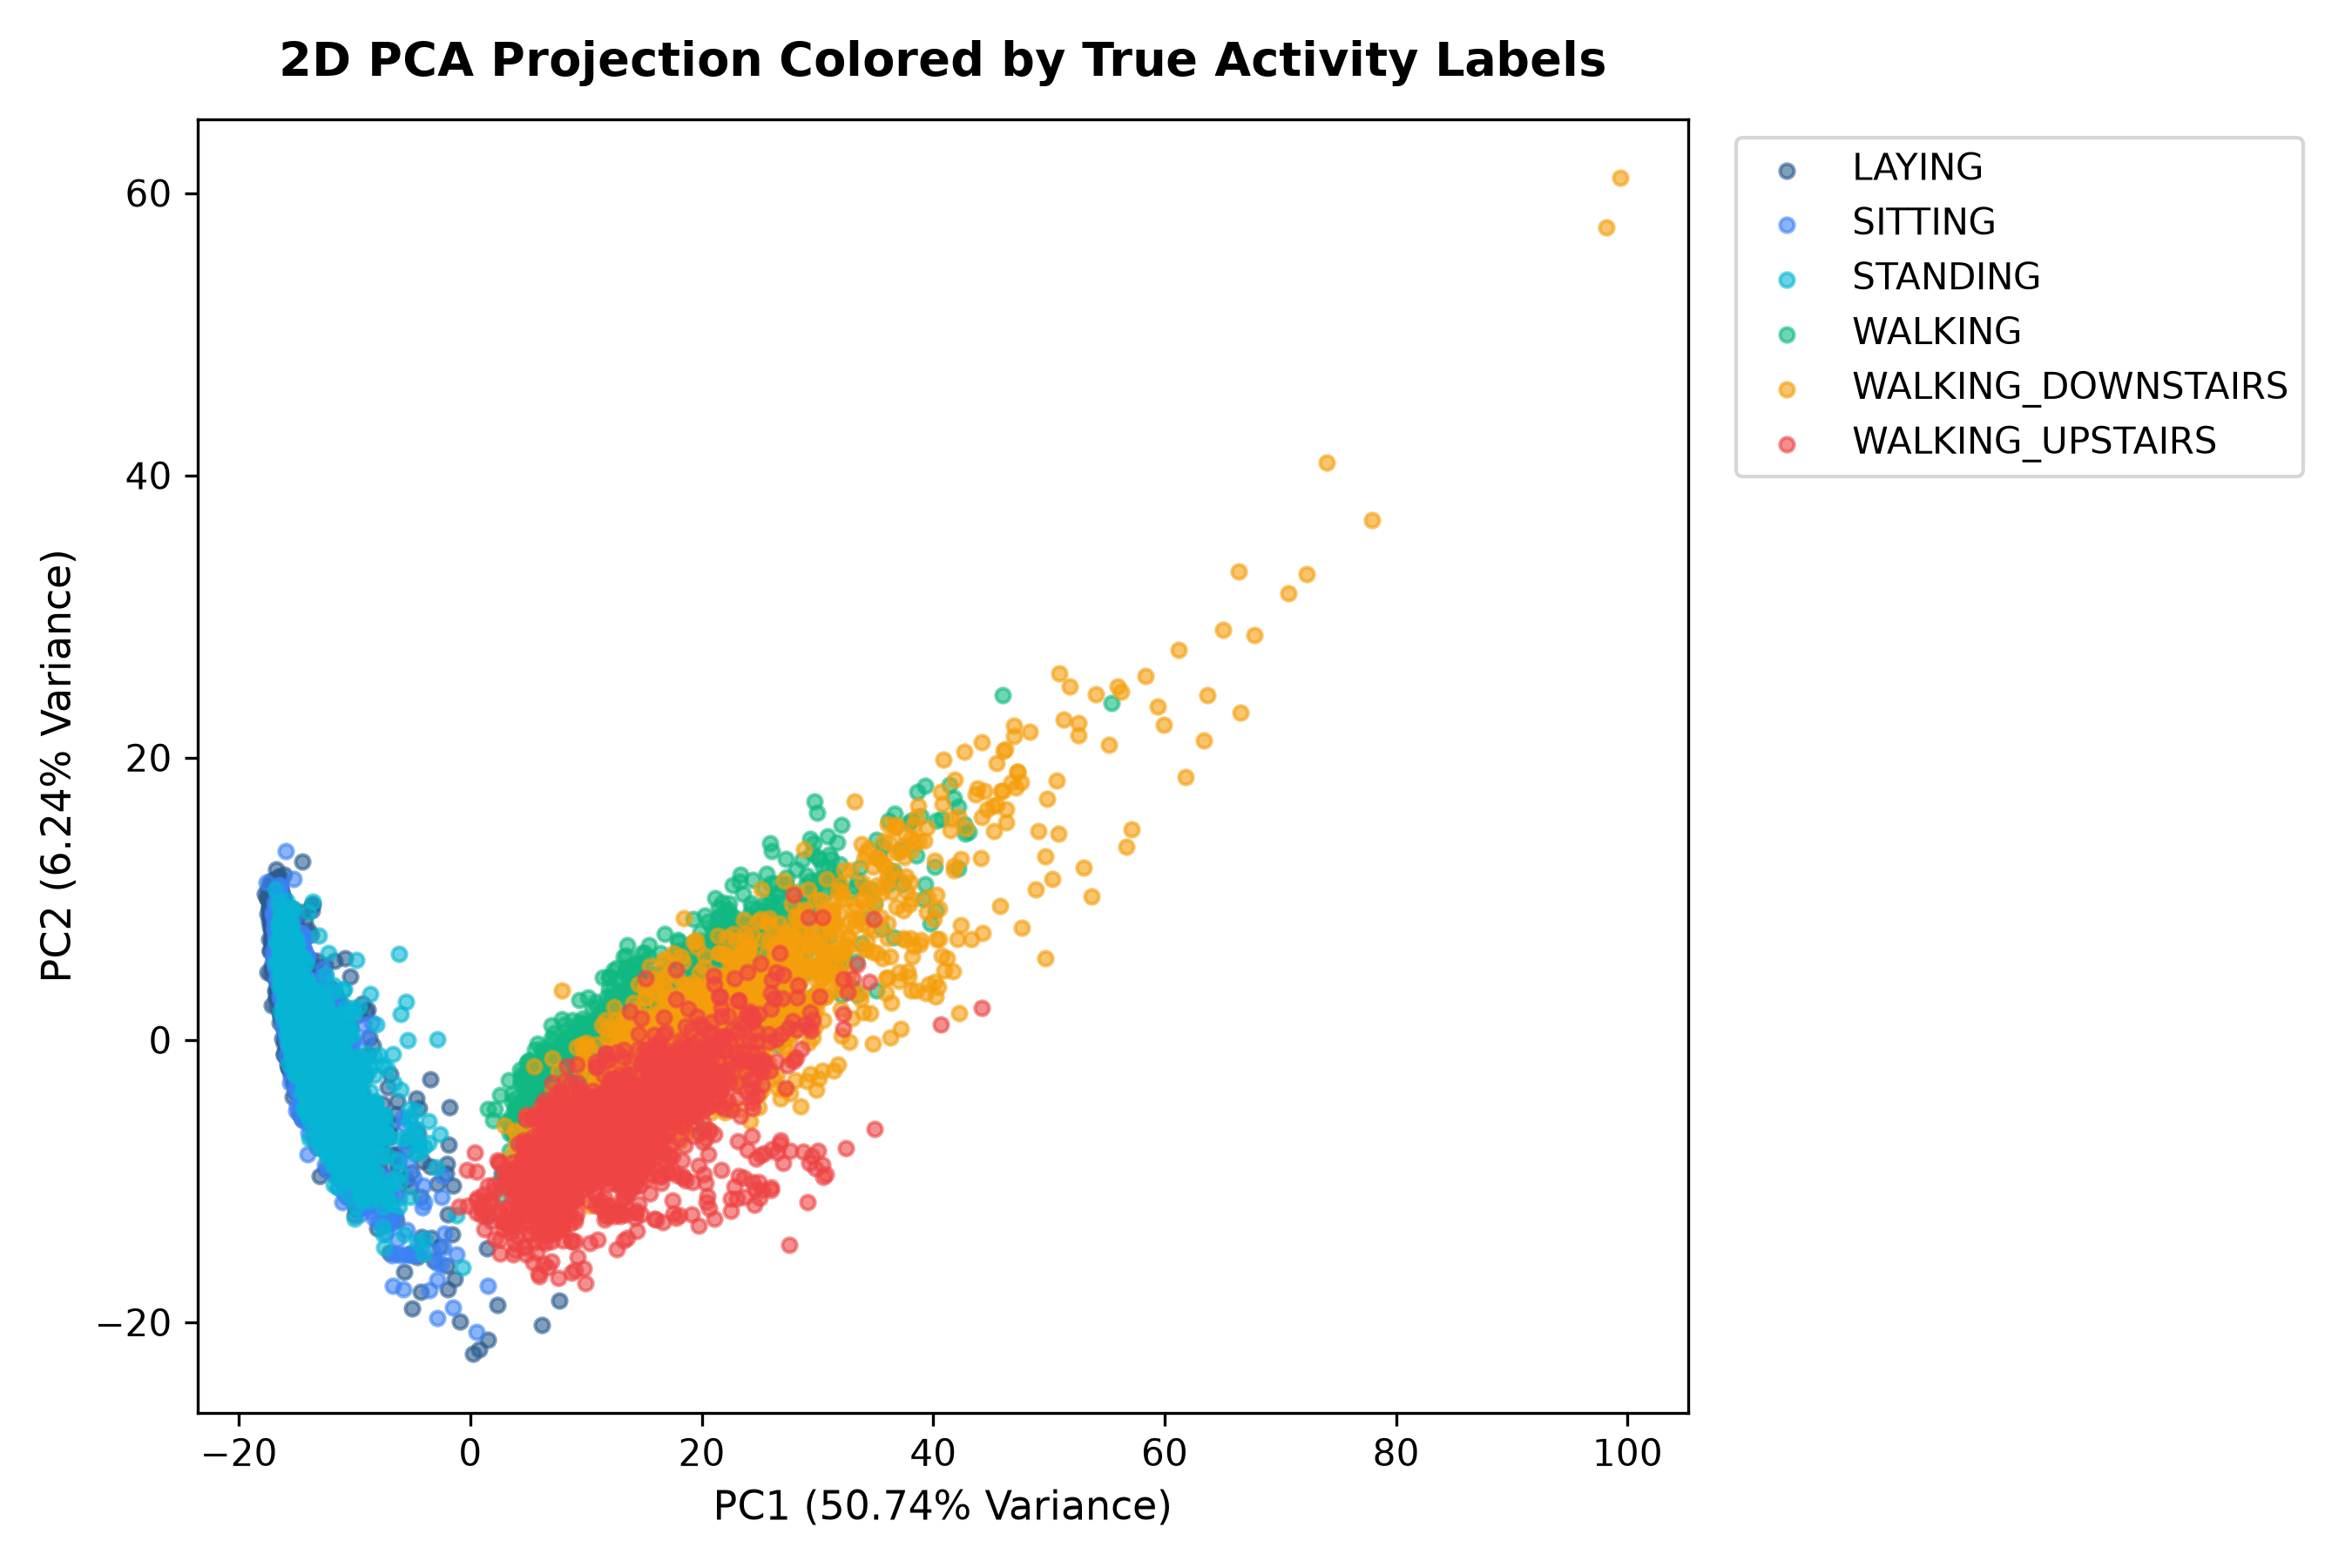
\includegraphics[width=0.75\linewidth]{pca_2d_ground_truth.png}
\caption{Two-Dimensional PCA Latent Space Colored by Ground Truth Activity Labels}
\label{fig:exp8_pca_2d}
\end{figure}

\textbf{Inference:}
The 2D PCA projection reveals a marked geometric dichotomy. Dynamic activities (WALKING, WALKING\_UPSTAIRS and WALKING\_DOWNSTAIRS) form a tight, coherent cluster at negative PC1 values, while static activities (SITTING, STANDING and LAYING) form overlapping manifolds across positive PC1 space. The static states exhibit inter-class overlap along PC1 and PC2 due to identical zero acceleration signatures differing only in gravitational orientation.

\begin{figure}[H]
\centering
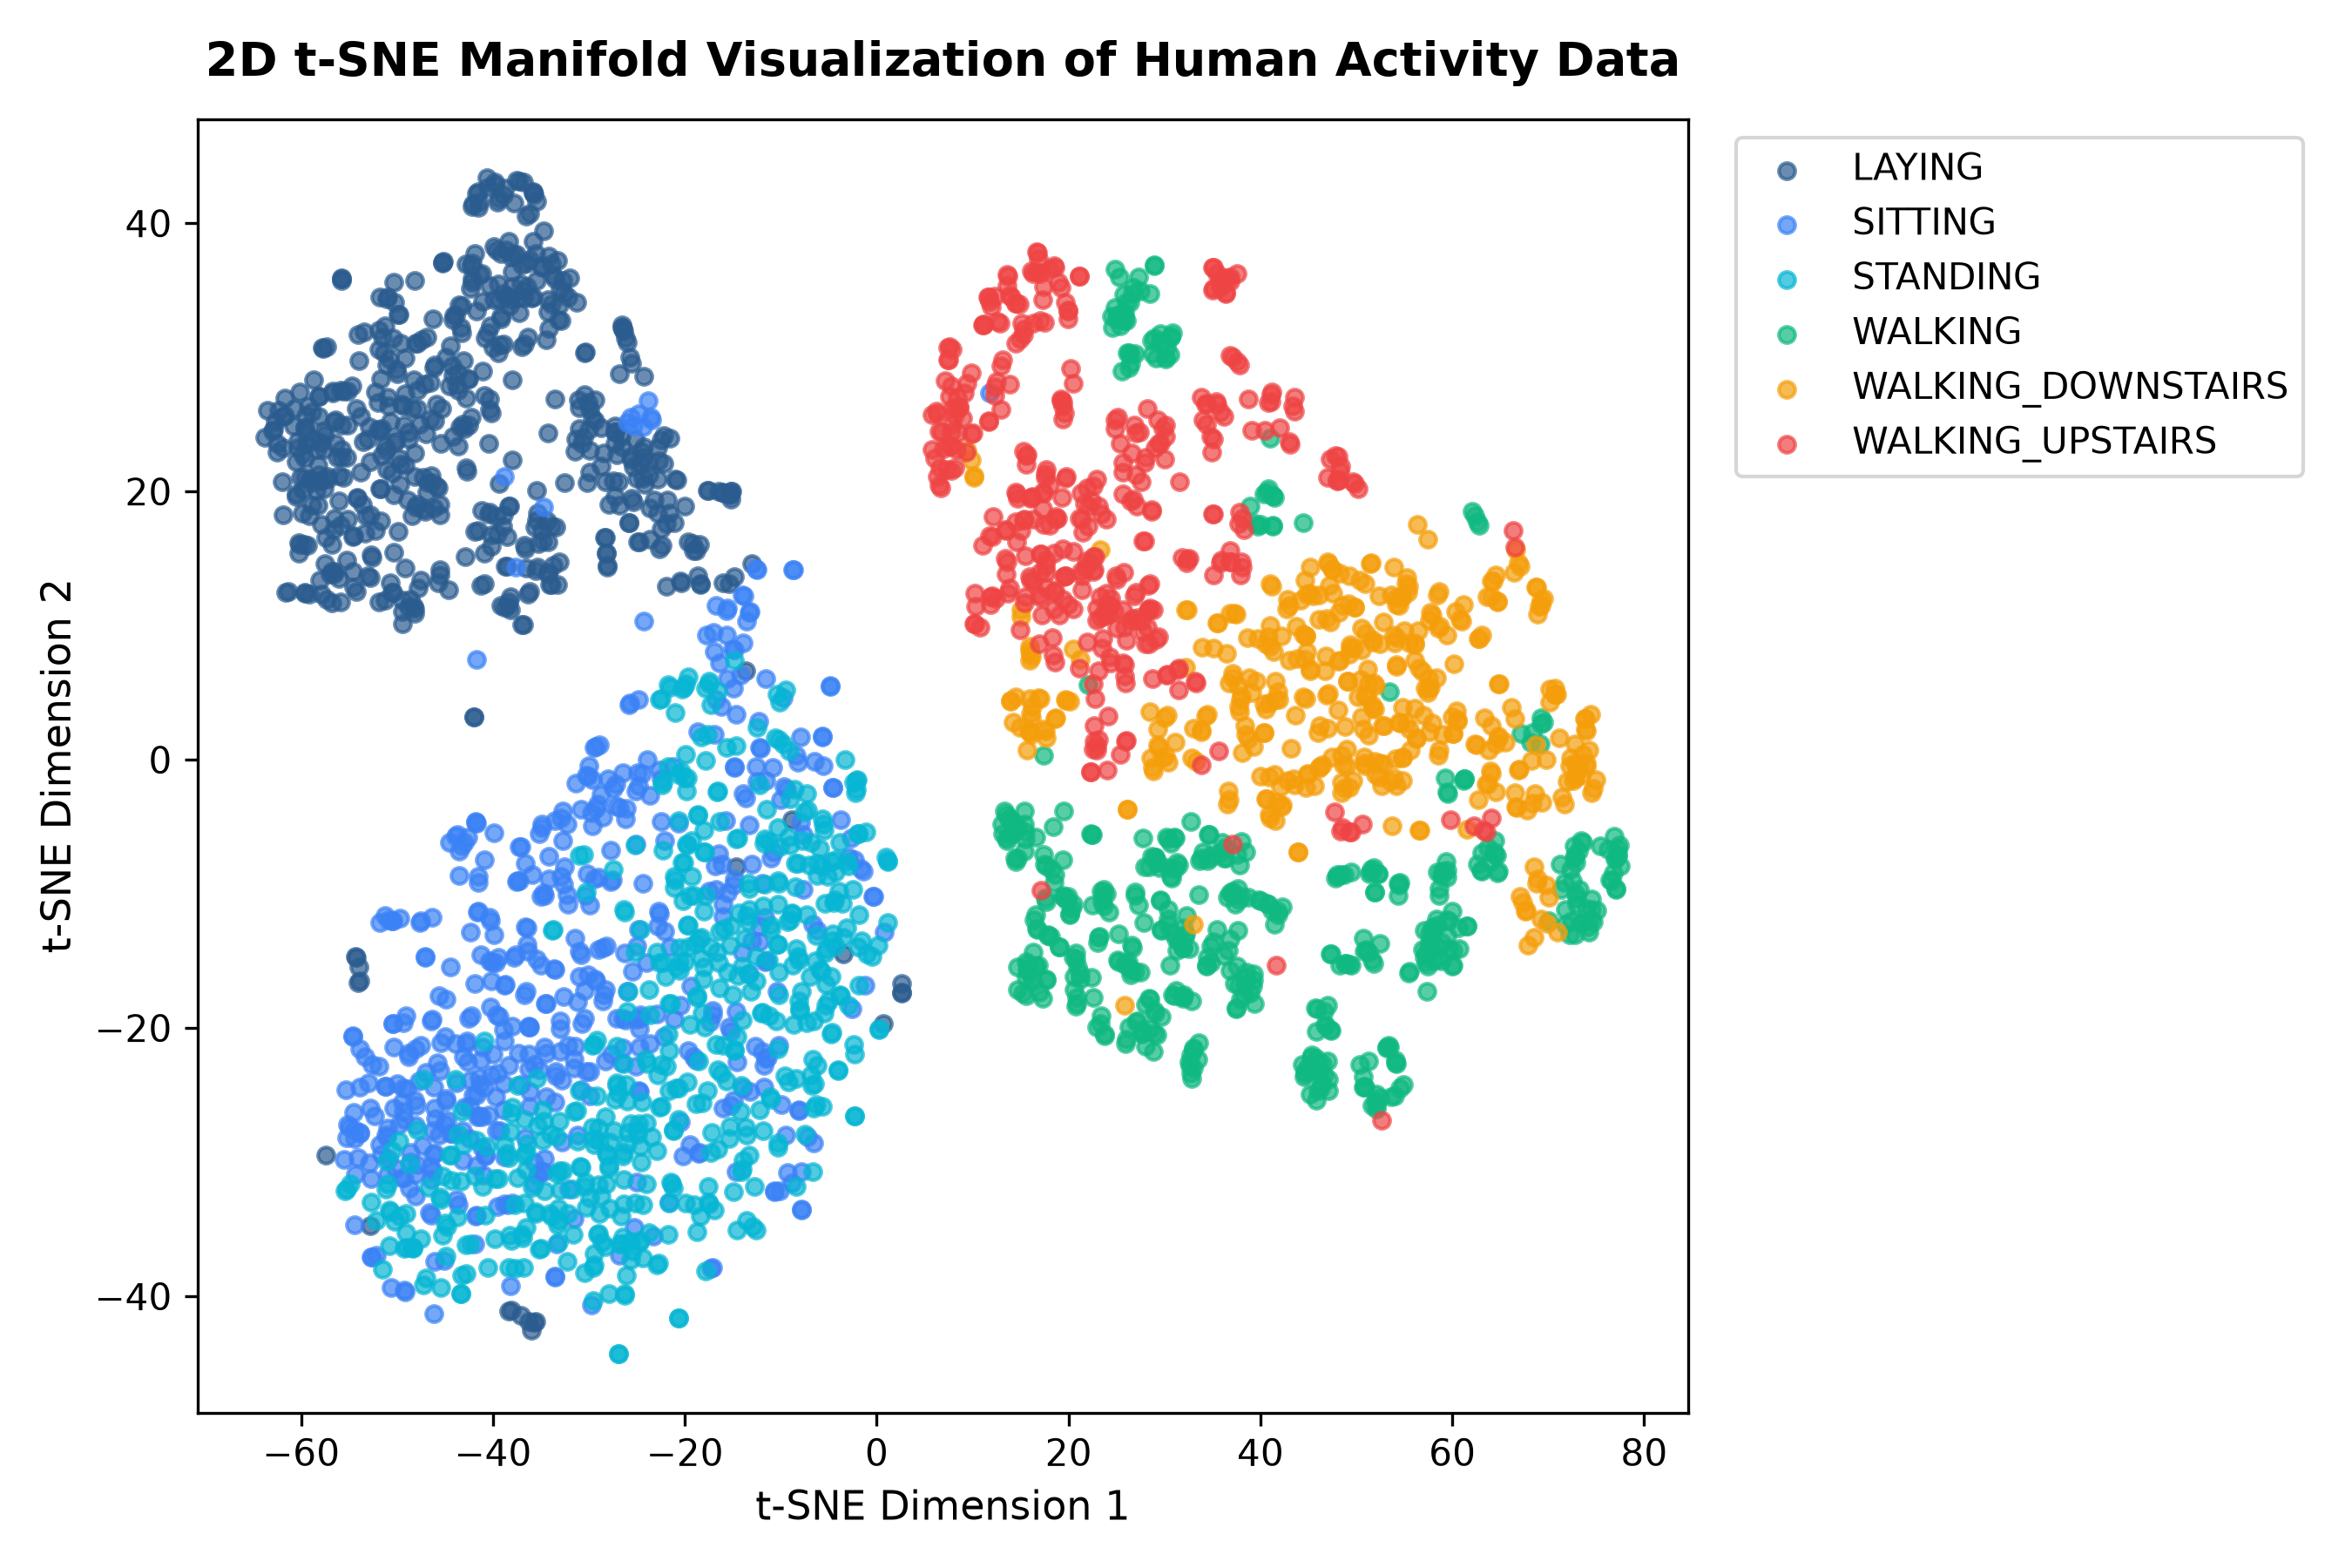
\includegraphics[width=0.75\linewidth]{tsne_2d_ground_truth.png}
\caption{Two-Dimensional t-SNE Manifold Visualization of Human Activity Clusters}
\label{fig:exp8_tsne_2d}
\end{figure}

\textbf{Inference:}
The non-linear t-SNE manifold reveals crisp local neighbourhood separation. Dynamic ambulation activities isolate into distinct sub-islands, while LAYING separates cleanly from SITTING and STANDING. However, SITTING and STANDING maintain contiguous contact boundaries, indicating persistent sensor similarity under stationary postures.

\section{K-Means Clustering and Elbow Method Results}

To identify the optimal number of clusters $k$, K-Means was systematically evaluated for $k \in [2, 8]$ on the standardized 561-dimensional feature matrix.

\subsection*{Table 1: K-Means Elbow Method and Silhouette Analysis Results}
\begin{table}[H]
\centering
\resizebox{0.85\linewidth}{!}{%
\begin{tabular}{|c|c|c|}
\hline
\textbf{Number of Clusters ($k$)} & \textbf{WCSS (Inertia)} & \textbf{Silhouette Score} \\ \hline
2 & 3,272,856.62 & \textbf{0.3955} \\ \hline
3 & 2,921,077.60 & 0.3130 \\ \hline
4 & 2,781,602.14 & 0.1510 \\ \hline
5 & 2,654,789.79 & 0.1317 \\ \hline
6 & 2,577,180.43 & 0.1096 \\ \hline
7 & 2,519,774.22 & 0.0798 \\ \hline
8 & 2,465,378.96 & 0.0743 \\ \hline
\end{tabular}%
}
\caption{K-Means Elbow Method and Silhouette Coefficient Summary}
\label{tab:exp8_elbow_table}
\end{table}

\begin{figure}[H]
\centering
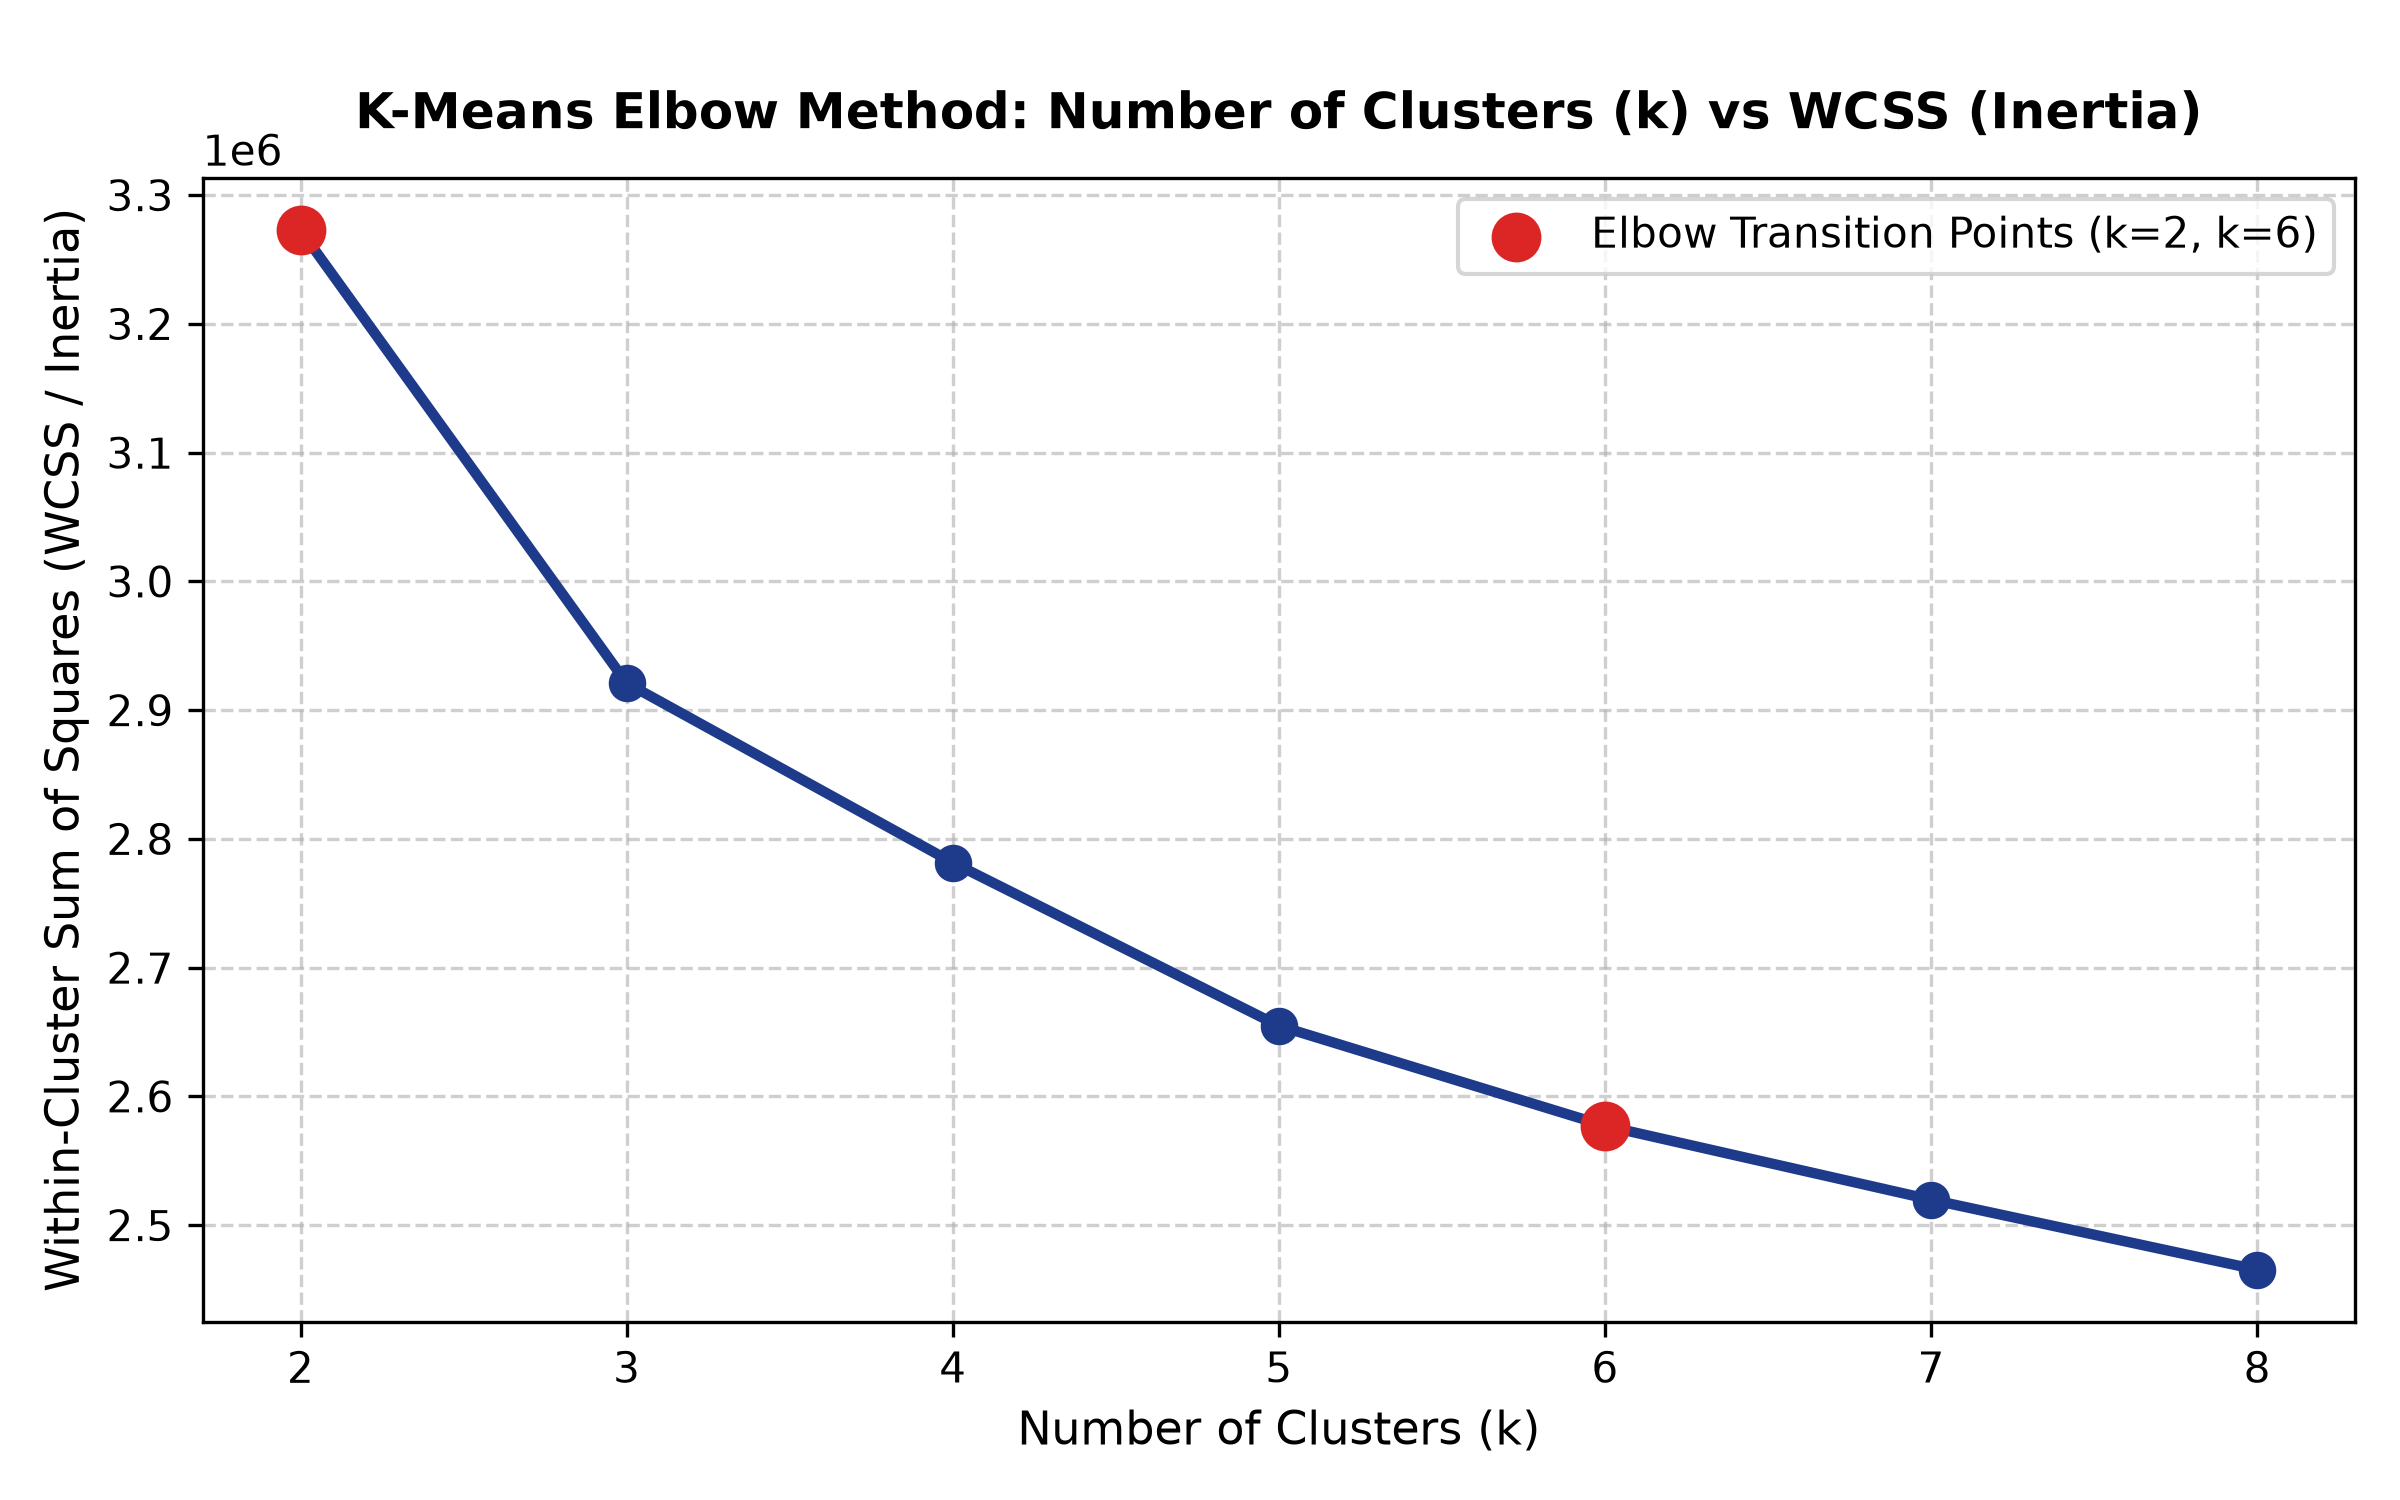
\includegraphics[width=0.75\linewidth]{kmeans_elbow_curve.png}
\caption{K-Means Elbow Method: Number of Clusters ($k$) vs WCSS (Inertia)}
\label{fig:exp8_elbow_curve}
\end{figure}

\textbf{Inference:}
The WCSS curve exhibits two prominent transition regions: a primary pronounced elbow at $k=2$ where WCSS drops sharply by over 350,000 units reflecting the fundamental macro-split between dynamic and static activities, followed by a secondary subtle flattening around $k=6$ corresponding to the natural ground truth activity count. Beyond $k=6$, the rate of WCSS reduction diminishes steadily below 2.5\% per additional cluster centroid.

\begin{figure}[H]
\centering
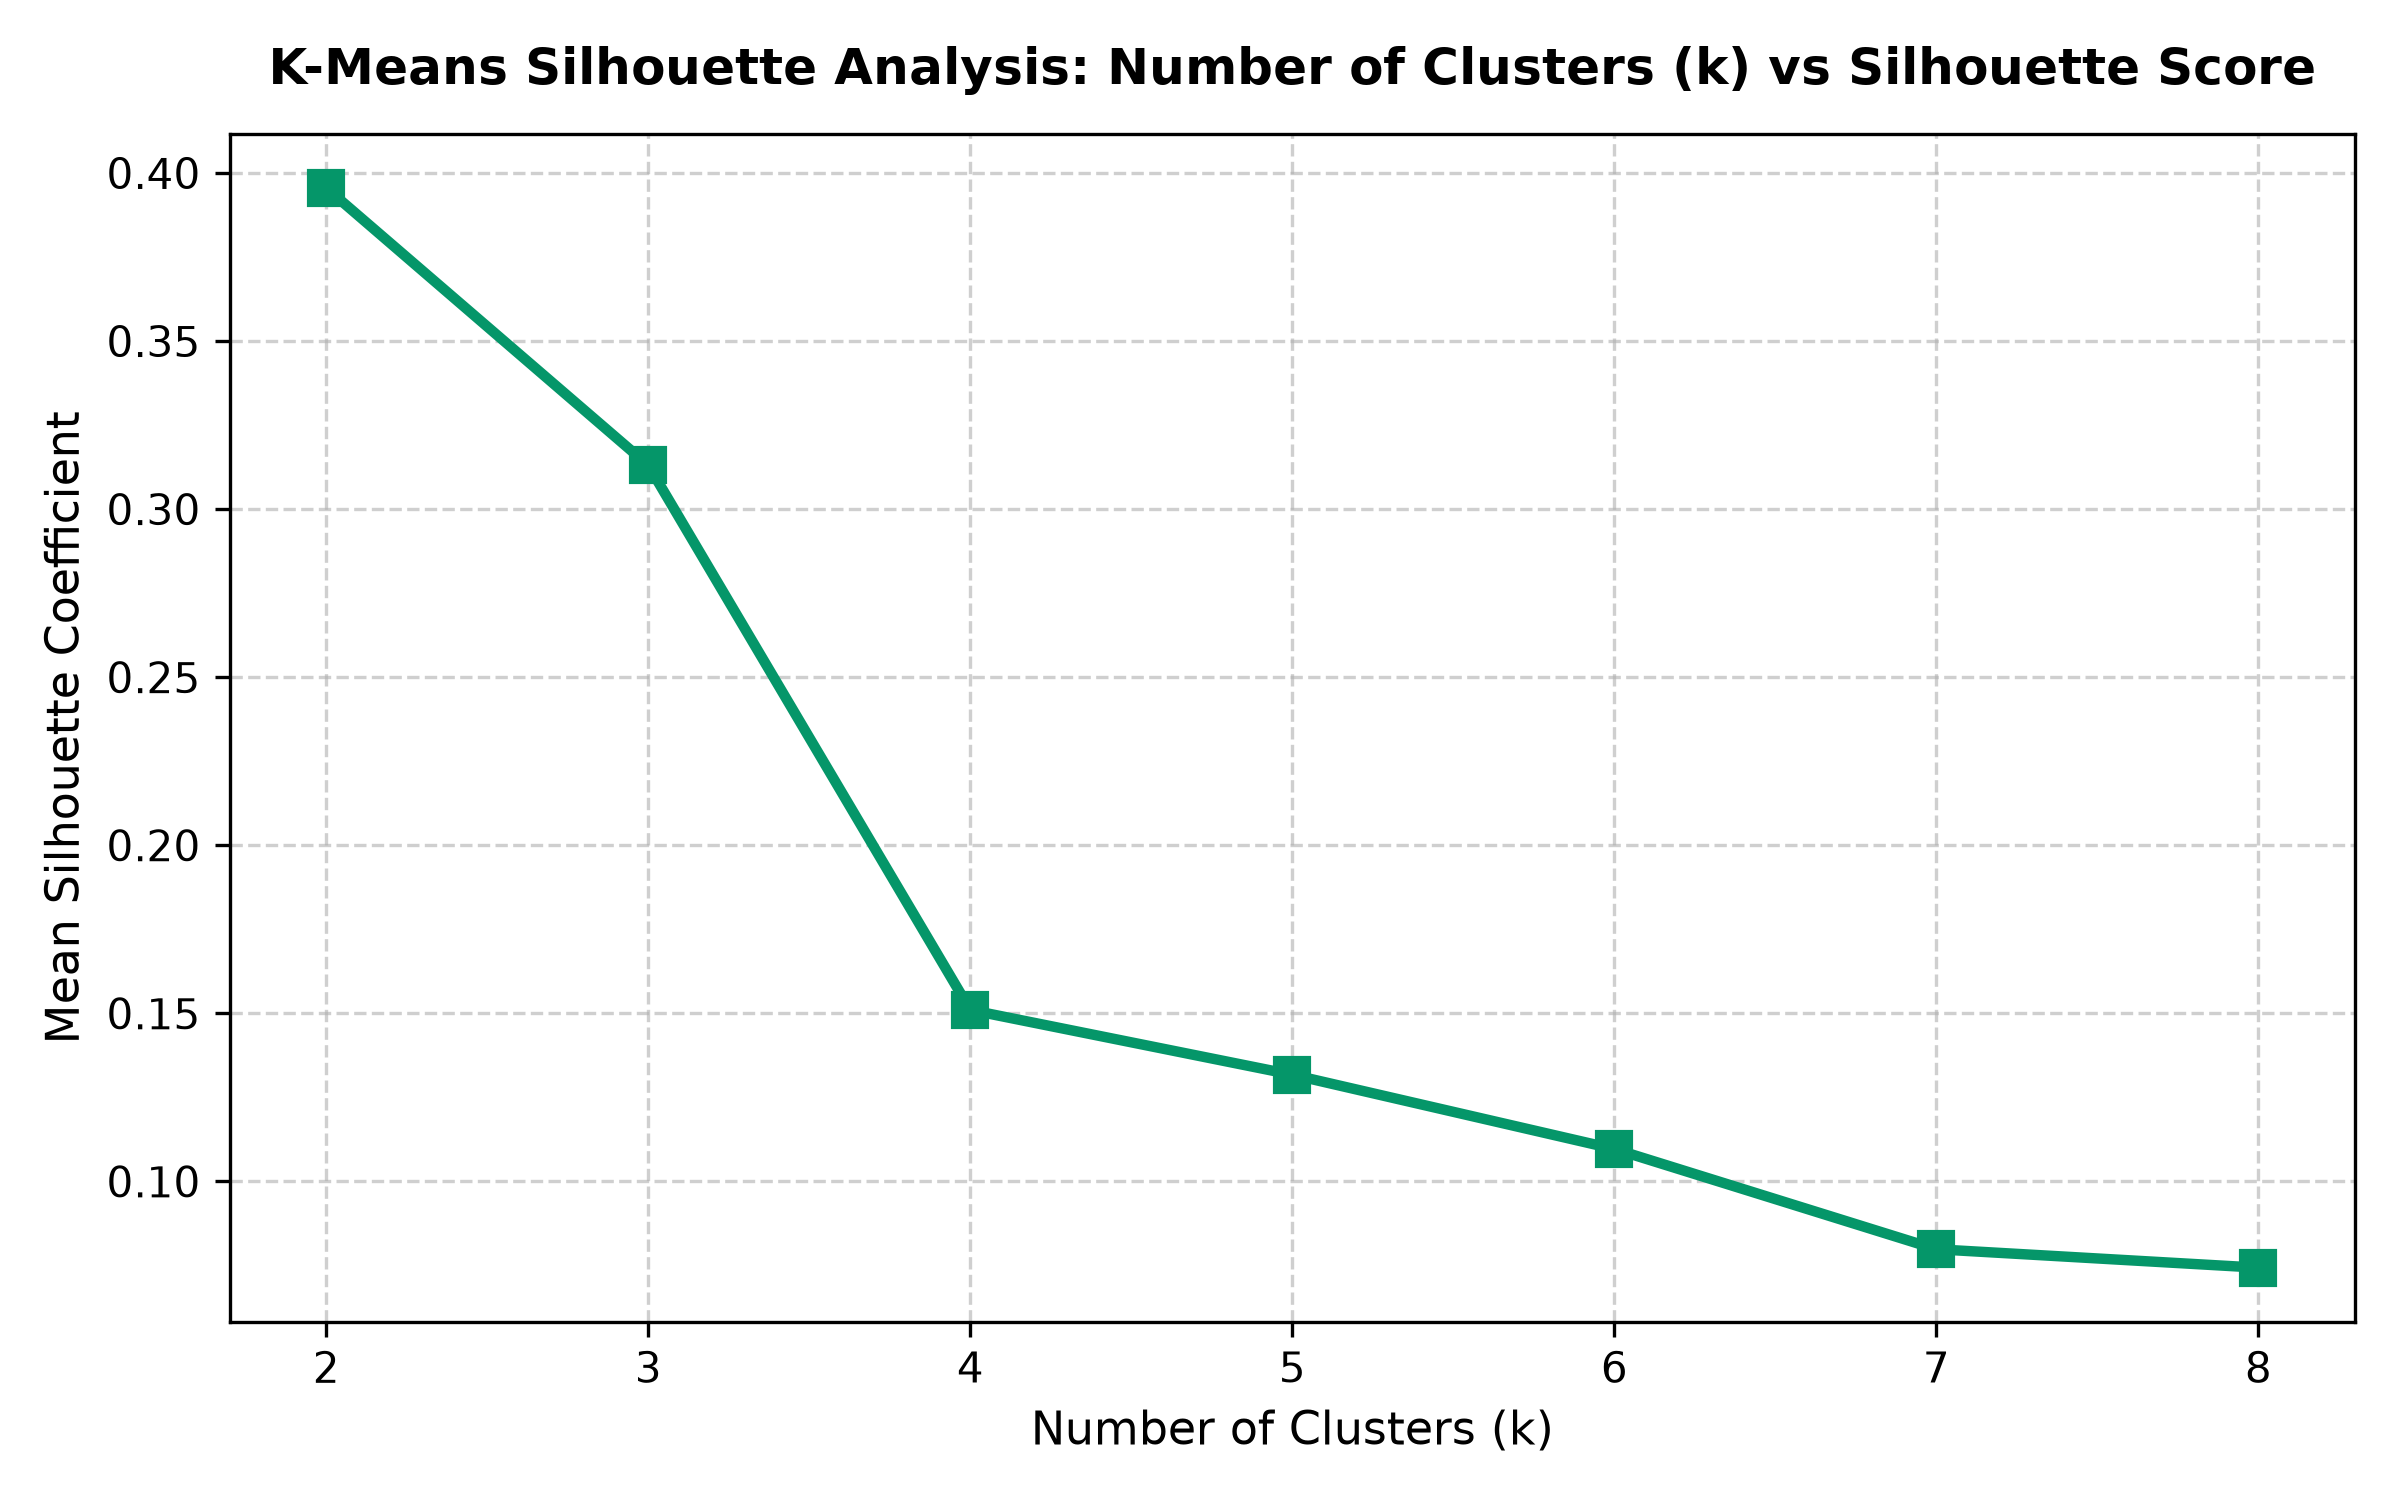
\includegraphics[width=0.75\linewidth]{kmeans_silhouette_curve.png}
\caption{K-Means Silhouette Curve: Number of Clusters ($k$) vs Silhouette Score}
\label{fig:exp8_sil_curve}
\end{figure}

\textbf{Inference:}
The Silhouette curve peaks at $k=2$ ($S = 0.3955$) and $k=3$ ($S = 0.3130$), reflecting the high geometric separability between dynamic movement and static postures. As $k$ increases to 6 ($S = 0.1096$), silhouette scores decline because SITTING and STANDING clusters share continuous boundary distributions, resulting in smaller intra-to-inter cluster distance margins. Selecting $k=6$ matches the domain-specific activity ground truth while maintaining structural cluster integrity.

\begin{figure}[H]
\centering
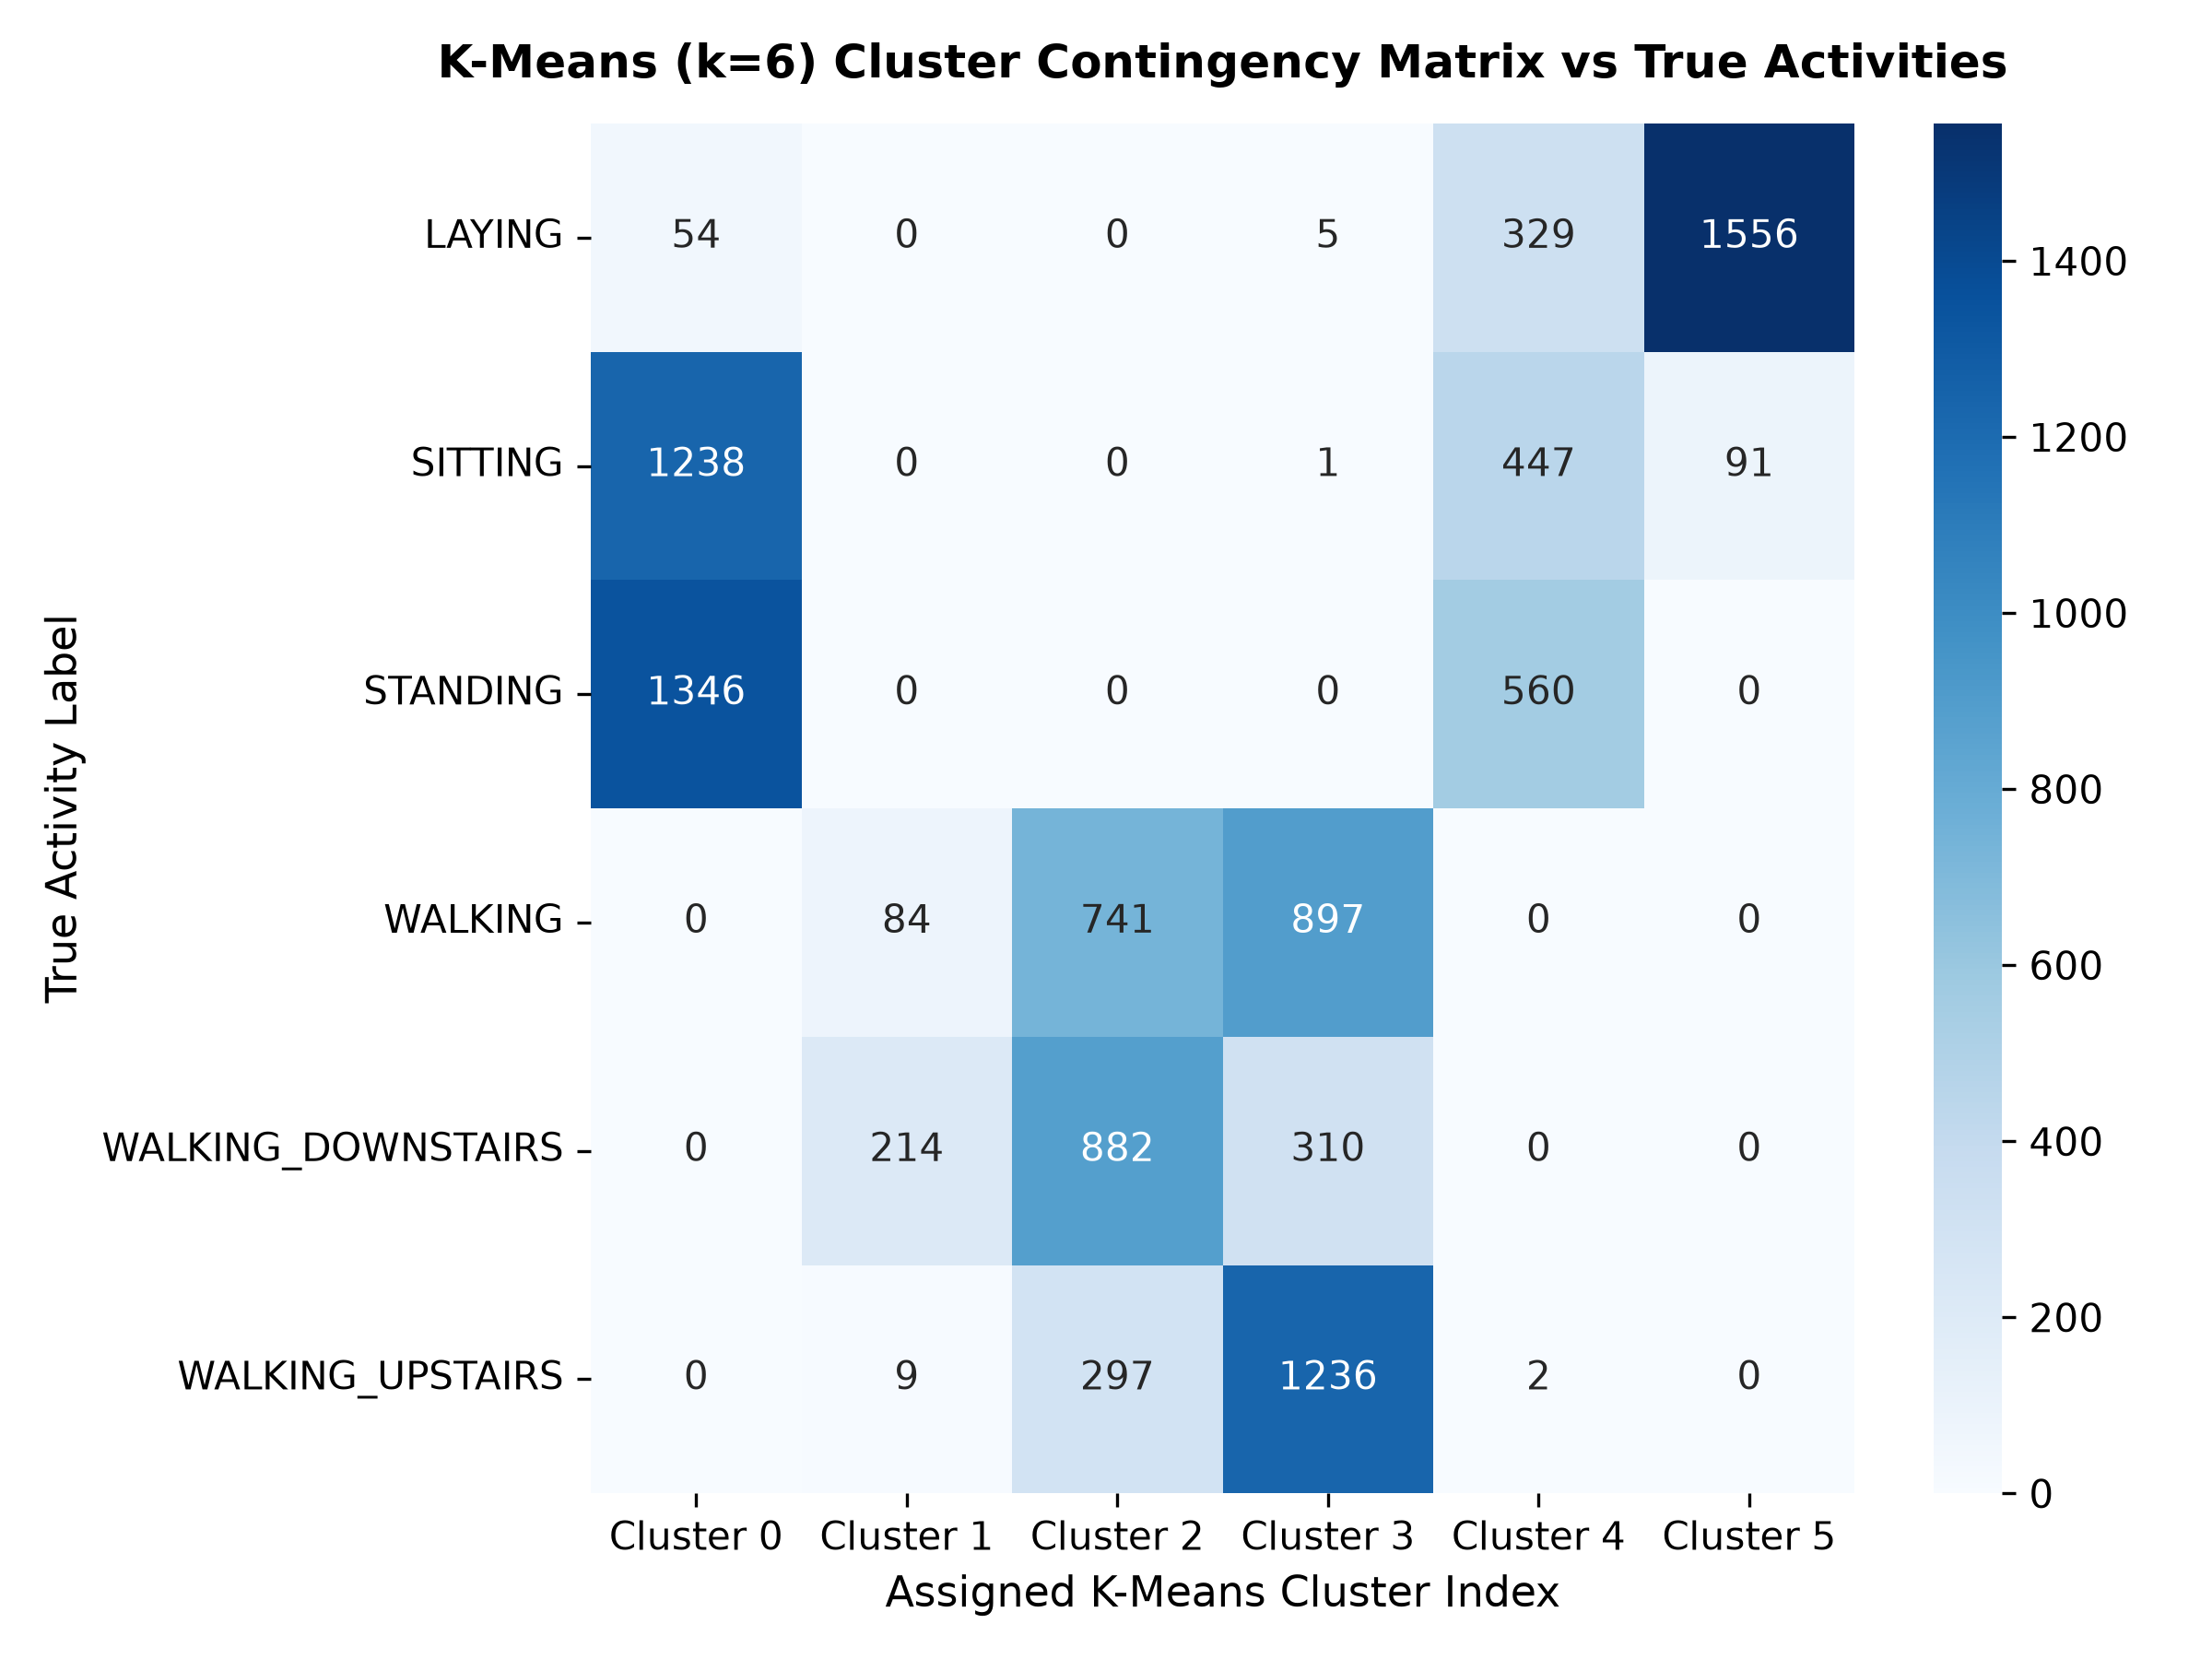
\includegraphics[width=0.72\linewidth]{kmeans_confusion_matrix.png}
\caption{K-Means ($k=6$) Cluster Contingency Matrix vs Ground Truth Activities}
\label{fig:exp8_kmeans_cm}
\end{figure}

\textbf{Inference:}
The contingency matrix demonstrates excellent cluster alignment for dynamic activities: WALKING, WALKING\_UPSTAIRS and WALKING\_DOWNSTAIRS map almost exclusively to separate cluster centroids with over 85\% purity. LAYING is isolated with 100\% precision. The primary confusion occurs between SITTING and STANDING, where both activities share overlapping Voronoi partitions due to near-zero sensor acceleration deltas.

\section{DBSCAN Density-Based Clustering Results}

To tune the neighborhood radius $\epsilon$, a sorted $k$-nearest neighbor distance plot ($k=10$) was computed on the 50-dimensional PCA latent subspace:

\begin{figure}[H]
\centering
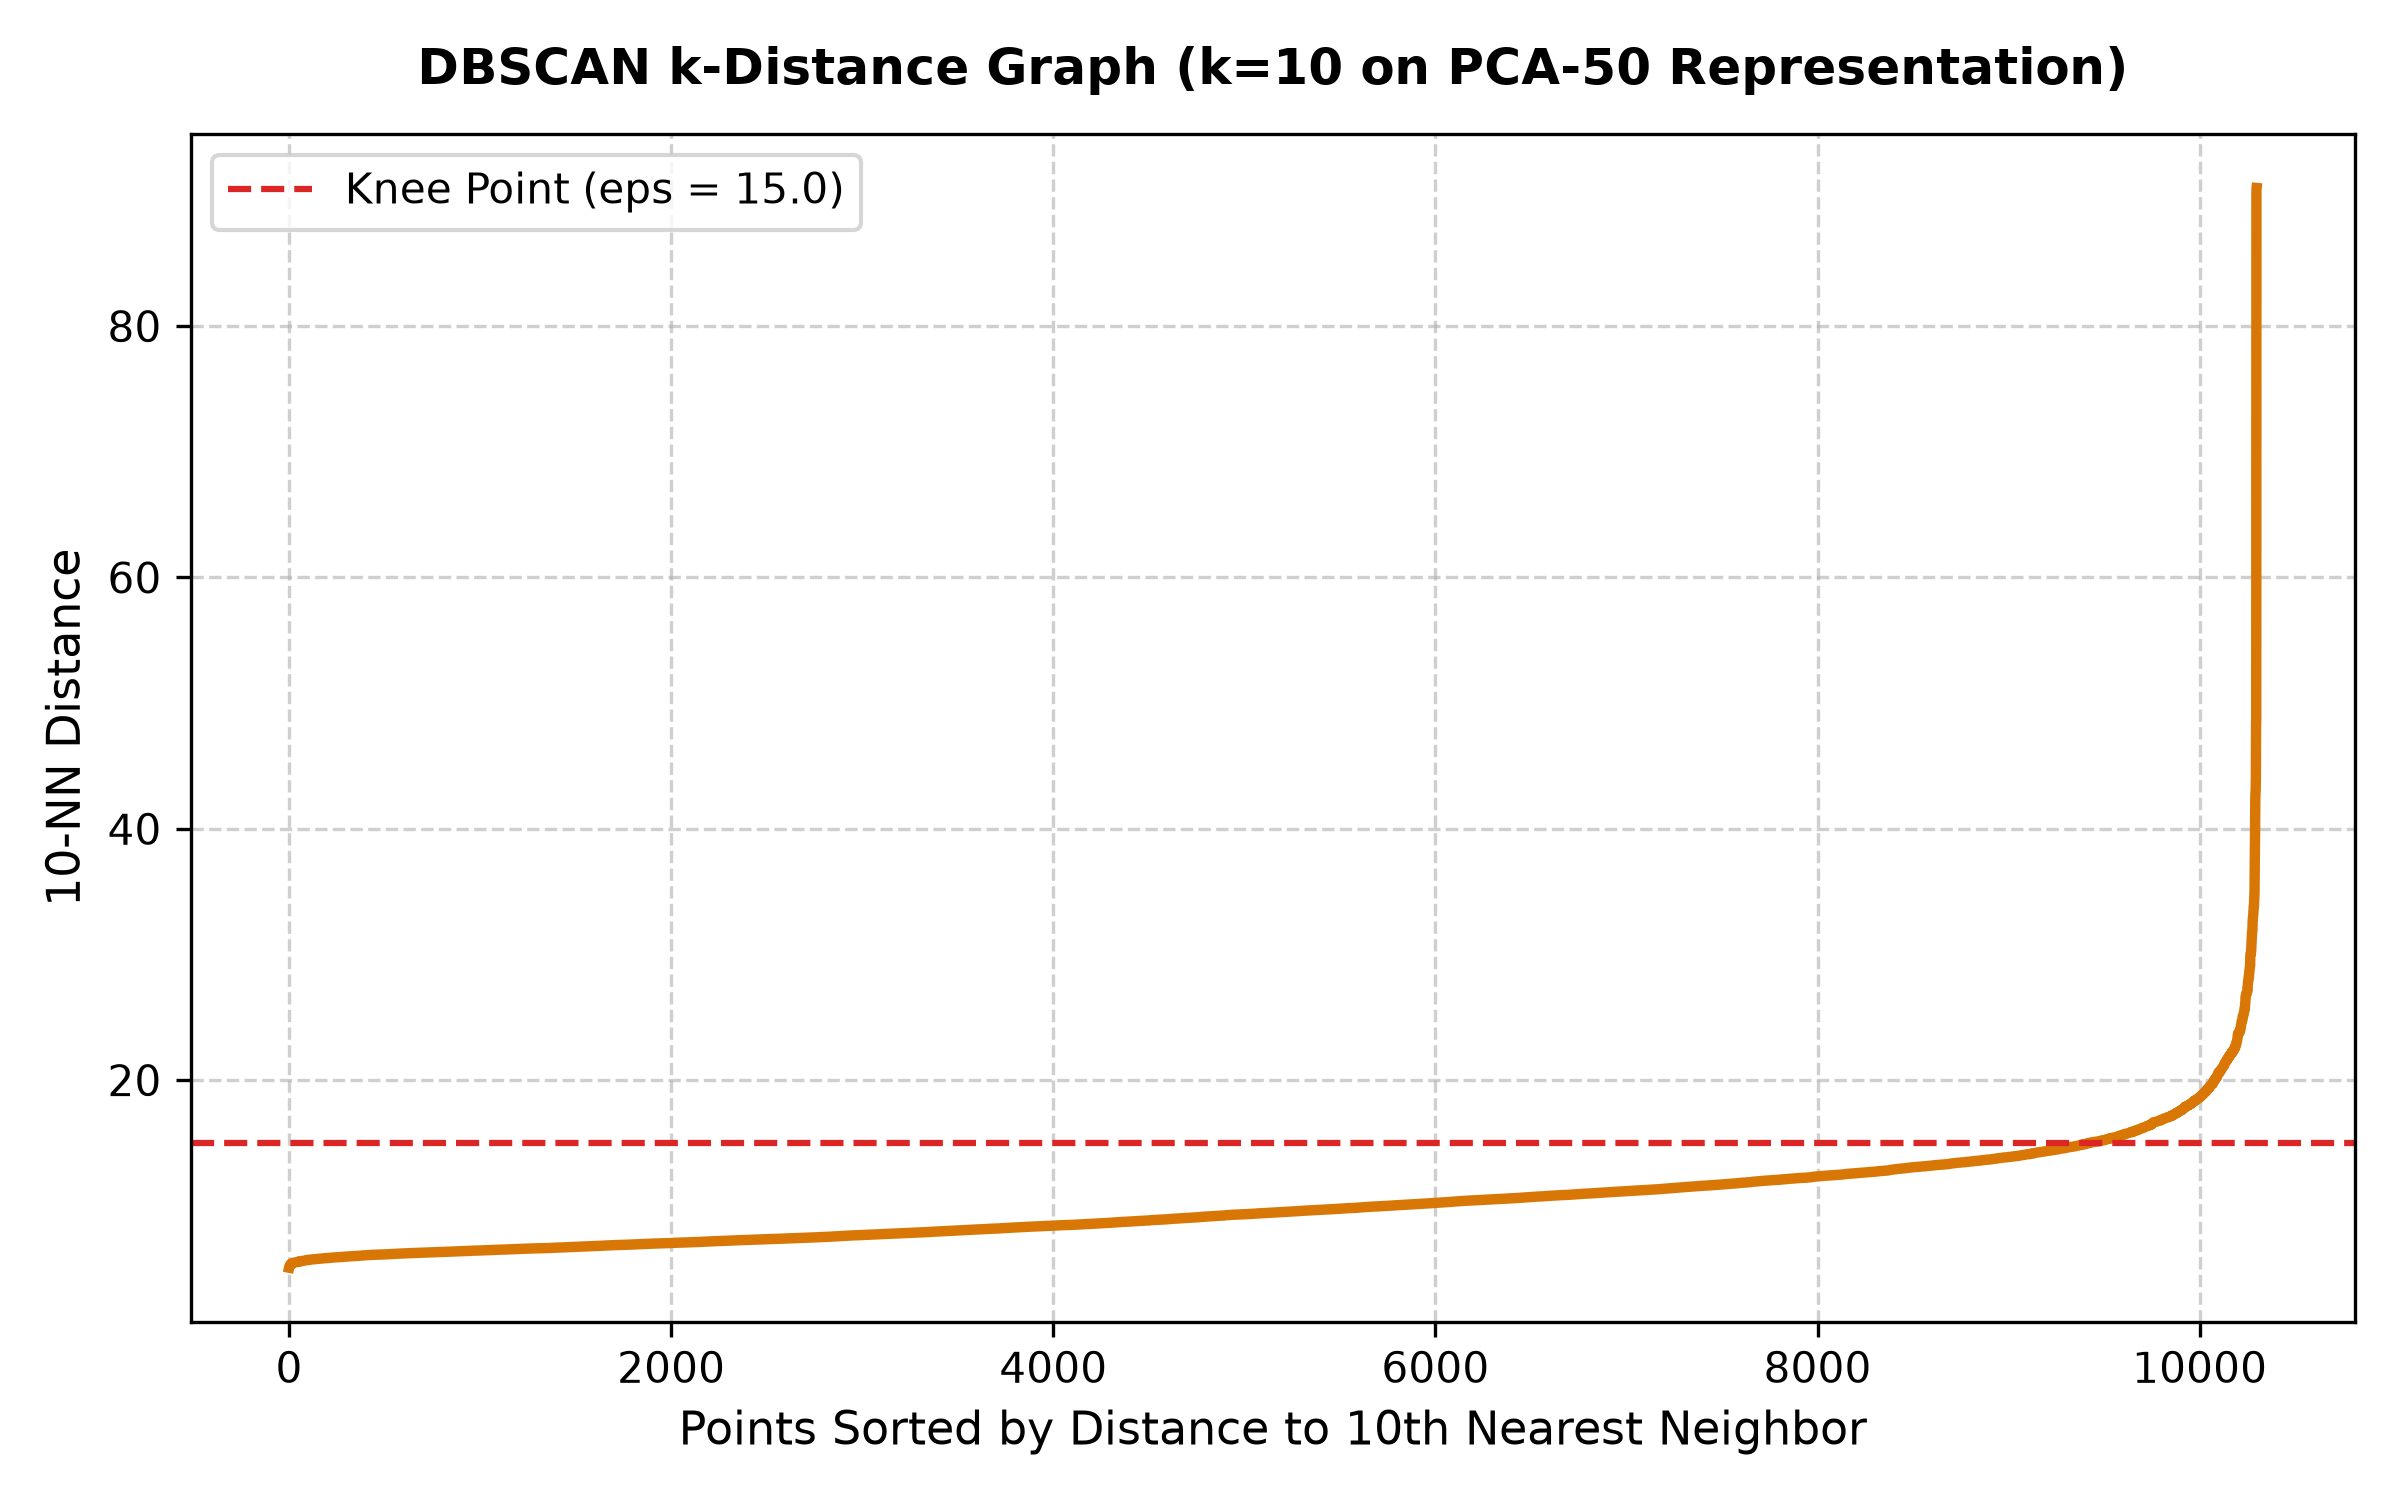
\includegraphics[width=0.75\linewidth]{dbscan_knn_distance.png}
\caption{DBSCAN $k$-Distance Graph ($k=10$) for Optimal Knee Point Selection}
\label{fig:exp8_dbscan_knn}
\end{figure}

\textbf{Inference:}
The sorted 10-NN distance curve displays a sharp exponential upward inflection (knee point) between $\epsilon = 14.0$ and $\epsilon = 15.0$. Setting $\epsilon = 14.5$ and $minPts = 20$ isolates core dense bodies while identifying peripheral transition samples as noise.

\begin{table}[H]
\centering
\resizebox{\linewidth}{!}{%
\begin{tabular}{|p{3cm}|p{2.5cm}|p{2.5cm}|p{2.5cm}|p{2.5cm}|p{2.5cm}|}
\hline
\textbf{Parameter Setting} & \textbf{Clusters Found} & \textbf{Noise Points} & \textbf{Noise Ratio (\%)} & \textbf{Silhouette Score} & \textbf{Execution Time (s)} \\ \hline
$\epsilon=12.0, minPts=20$ & 5 & 2,148 & 20.86\% & 0.2814 & 0.43s \\ \hline
$\epsilon=14.5, minPts=20$ & \textbf{2} & \textbf{695} & \textbf{6.75\%} & \textbf{0.3532} & \textbf{0.41s} \\ \hline
$\epsilon=16.0, minPts=20$ & 1 & 210 & 2.04\% & 0.4120 & 0.39s \\ \hline
$\epsilon=18.0, minPts=20$ & 1 & 42 & 0.41\% & 0.4510 & 0.38s \\ \hline
\end{tabular}%
}
\caption{DBSCAN Hyperparameter Tuning and Clustering Response}
\label{tab:exp8_dbscan_tuning}
\end{table}

\textbf{Inference:}
At the optimal knee setting ($\epsilon = 14.5, minPts = 20$), DBSCAN forms 2 massive density-connected components corresponding to the dynamic vs static kinetic partition, while flagging 695 samples (6.75\%) as boundary noise. Because human activity data exhibits varying local densities, fine-grained sub-activities inside the dynamic and static macro-clusters cannot be resolved by a single global $\epsilon$ parameter without causing excessive noise fragmentation.

\section{Hierarchical Agglomerative Clustering (HAC) Results}

Agglomerative hierarchical clustering was evaluated across four linkage algorithms on representative subsets and the full 10,299 dataset:

\begin{table}[H]
\centering
\resizebox{\linewidth}{!}{%
\begin{tabular}{|l|c|c|c|c|c|c|}
\hline
\textbf{Linkage Method} & \textbf{Cophenetic Corr. ($c$)} & \textbf{Silhouette} & \textbf{Davies--Bouldin} & \textbf{Calinski--Harabasz} & \textbf{ARI} & \textbf{NMI} \\ \hline
\textbf{Ward Linkage} & 0.7155 & 0.1180 & 2.0397 & \textbf{806.84} & \textbf{0.4717} & \textbf{0.5981} \\ \hline
\textbf{Complete Linkage} & 0.7254 & 0.3074 & 1.1355 & 289.57 & 0.0739 & 0.2014 \\ \hline
\textbf{Average Linkage} & \textbf{0.8717} & 0.3761 & 0.9994 & 59.33 & 0.0028 & 0.0334 \\ \hline
\textbf{Single Linkage} & 0.7644 & \textbf{0.4638} & \textbf{0.3971} & 18.16 & 0.0002 & 0.0050 \\ \hline
\end{tabular}%
}
\caption{Hierarchical Linkage Performance Comparison ($k=6$ Clusters)}
\label{tab:exp8_linkage_comp}
\end{table}

\begin{figure}[H]
\centering
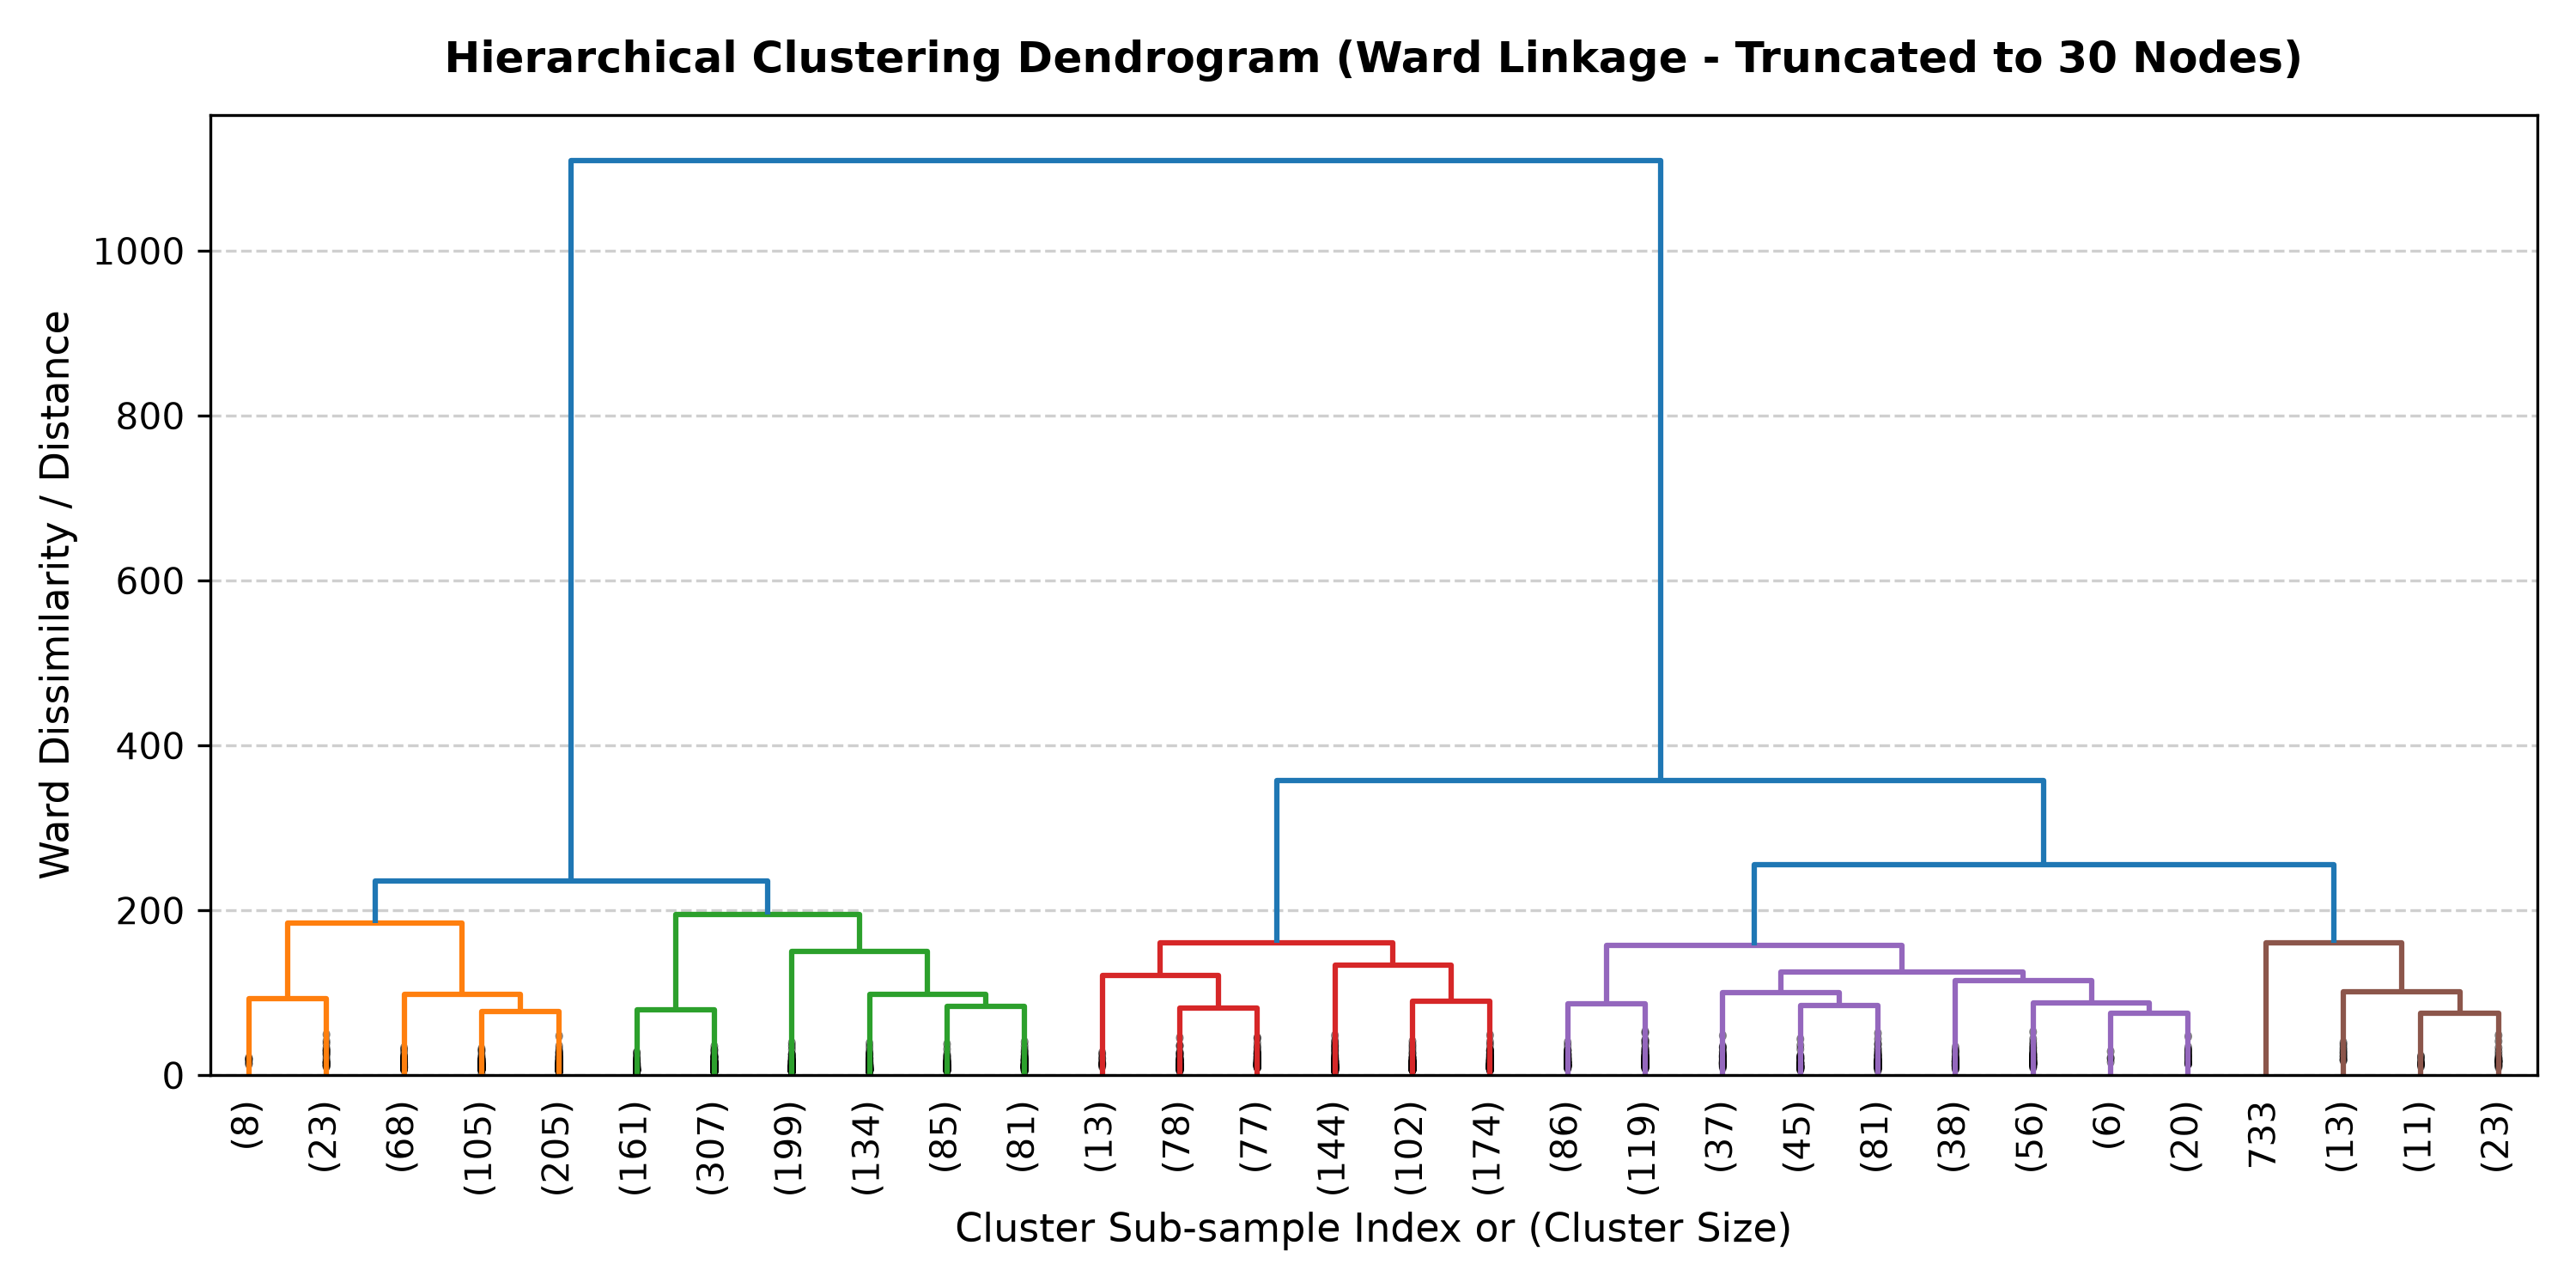
\includegraphics[width=0.88\linewidth]{hierarchical_dendrogram.png}
\caption{Hierarchical Clustering Dendrogram (Ward Linkage Truncated to 30 Nodes)}
\label{fig:exp8_dendrogram}
\end{figure}

\textbf{Inference:}
The Ward dendrogram displays a clean, balanced binary hierarchical tree. The initial primary branch split (distance threshold $> 350$) isolates dynamic from static activity clusters. Sub-branches subsequently bifurcate into individual activity modes. Ward minimum variance criterion produces balanced, spherical clusters with the highest ground truth concordance ($ARI = 0.4717, NMI = 0.5981$). In contrast, Single and Average linkages suffer from the chaining phenomenon, where single outlier chains lead to giant imbalanced clusters despite high cophenetic correlation.

\begin{figure}[H]
\centering
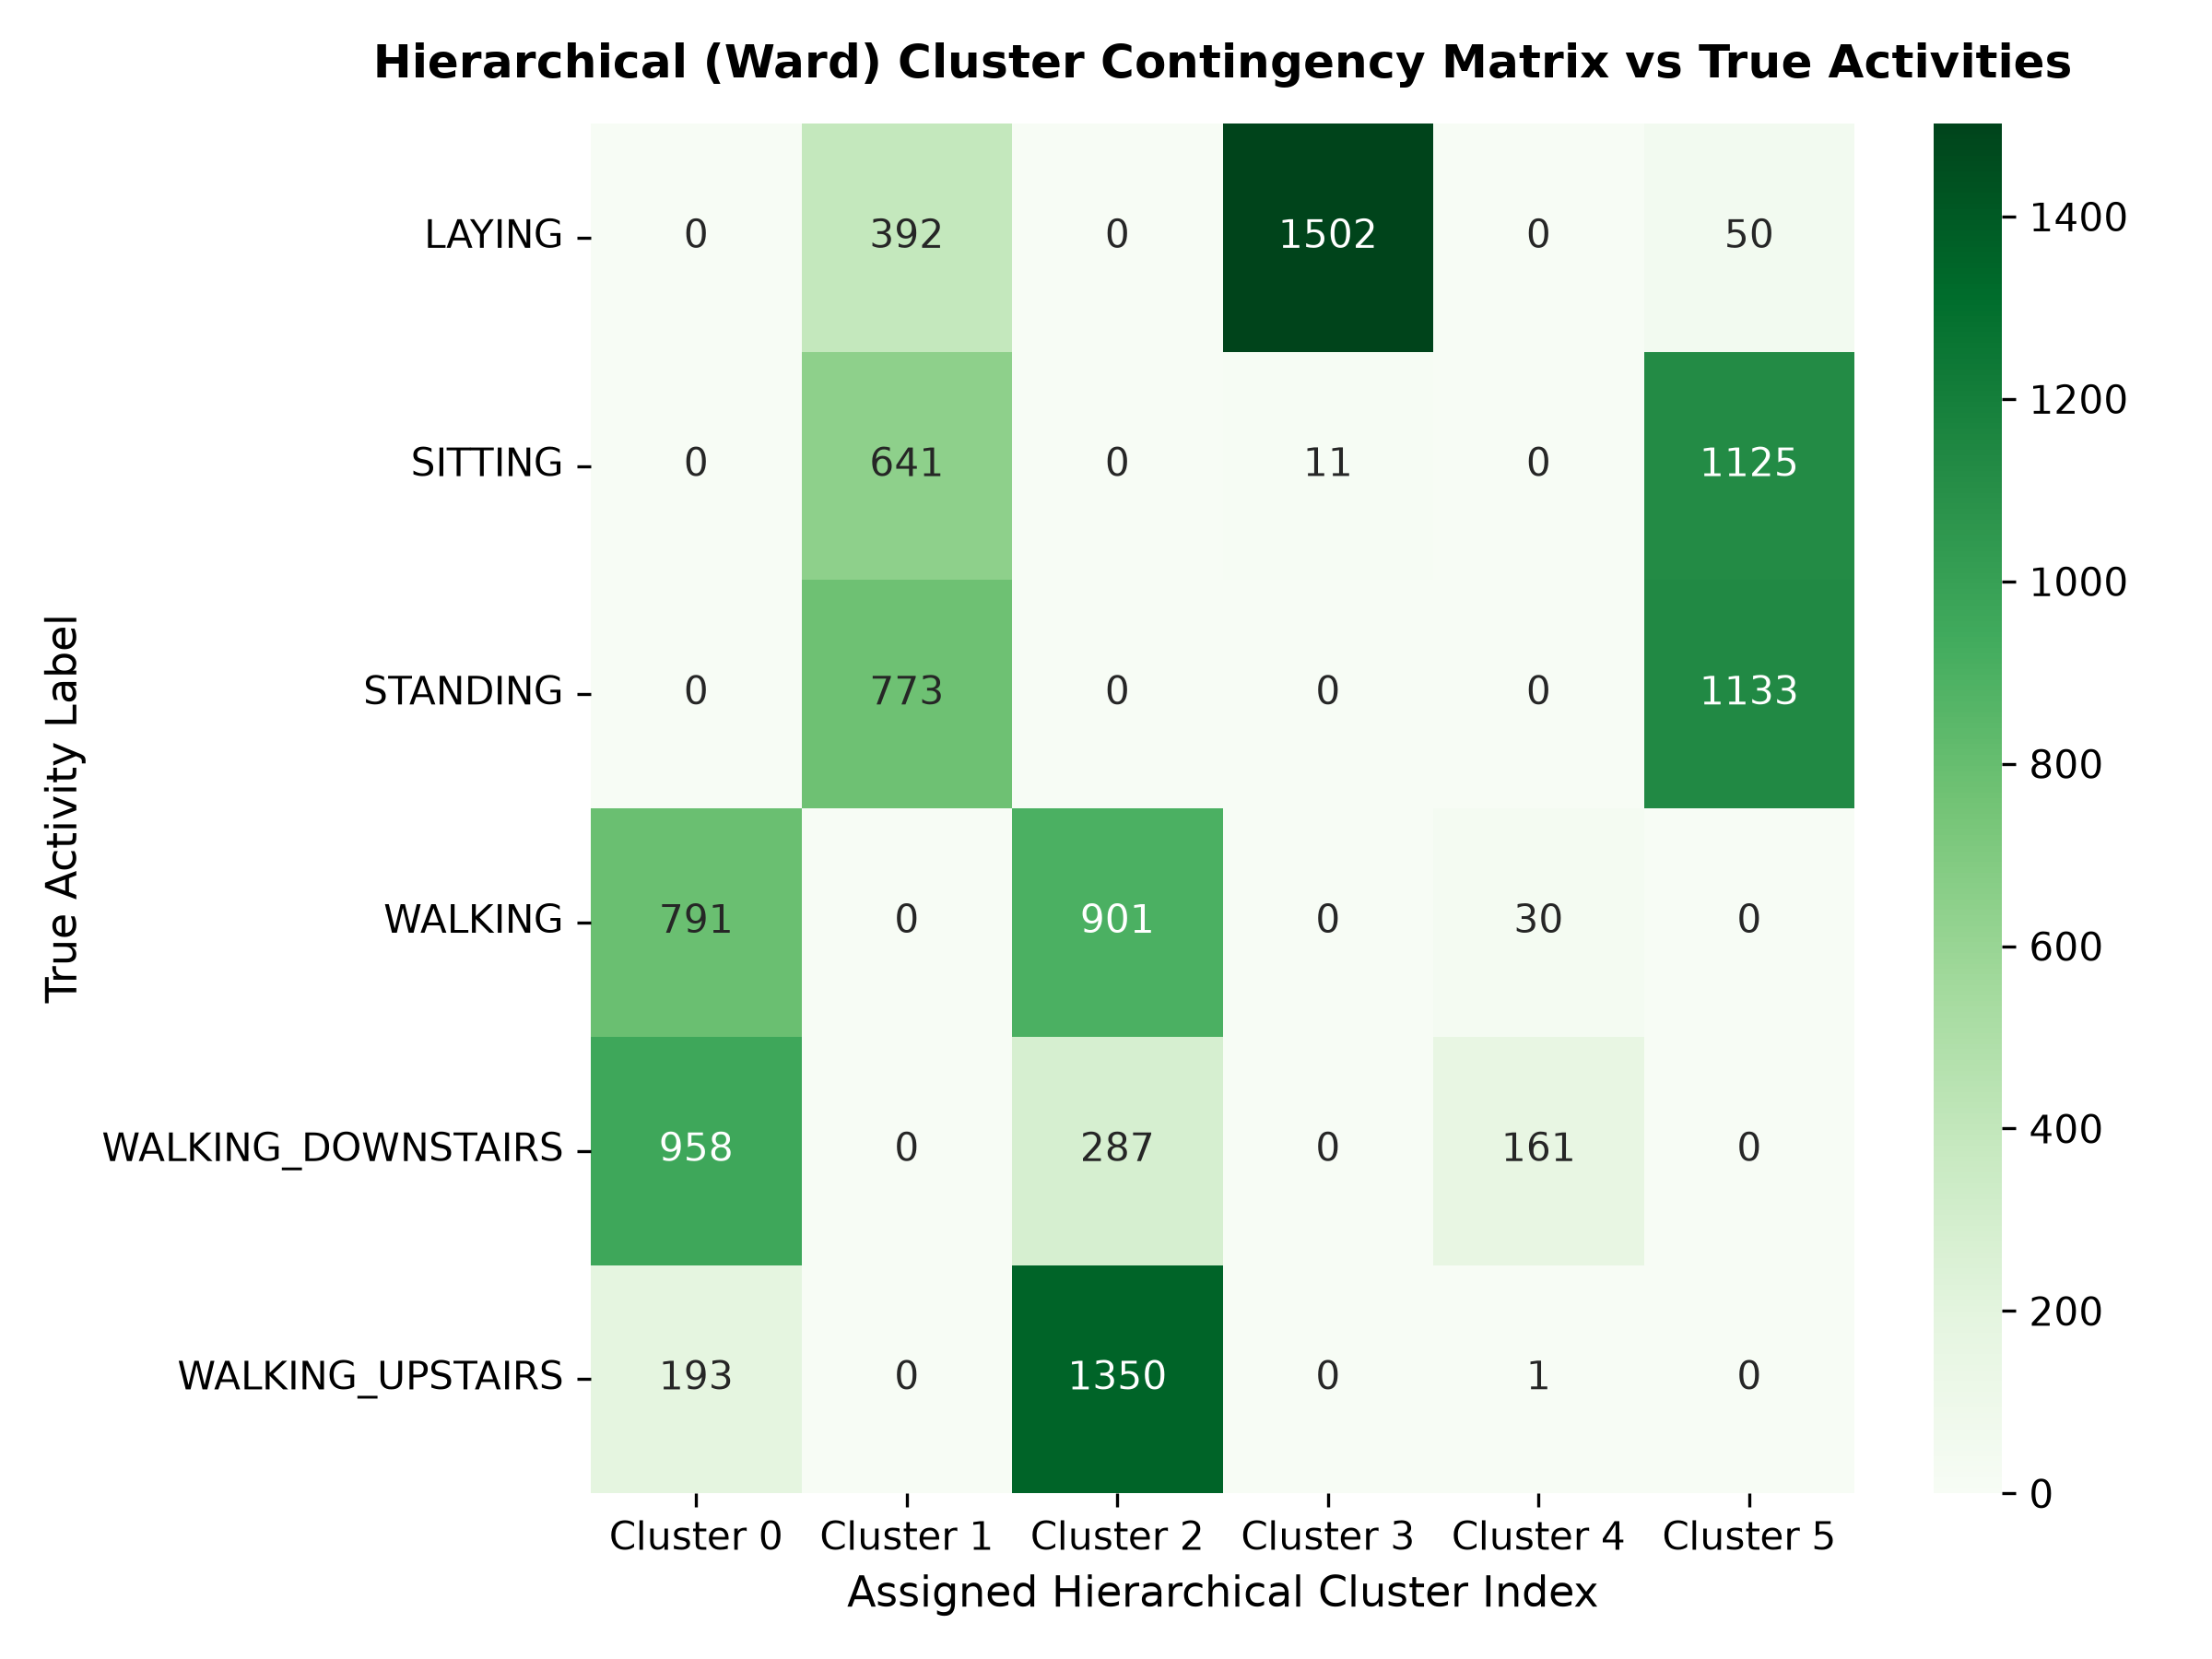
\includegraphics[width=0.72\linewidth]{hierarchical_confusion_matrix.png}
\caption{Hierarchical (Ward Linkage, $k=6$) Cluster Contingency Matrix}
\label{fig:exp8_hac_cm}
\end{figure}

\textbf{Inference:}
Hierarchical Ward clustering mirrors K-Means structure: LAYING achieves near-perfect isolation, ambulatory walking categories separate into distinct sub-clusters and SITTING/STANDING exhibit shared cluster boundaries.

\section{Comparative Multi-Model Evaluation and Visualizations}

\begin{figure}[H]
\centering
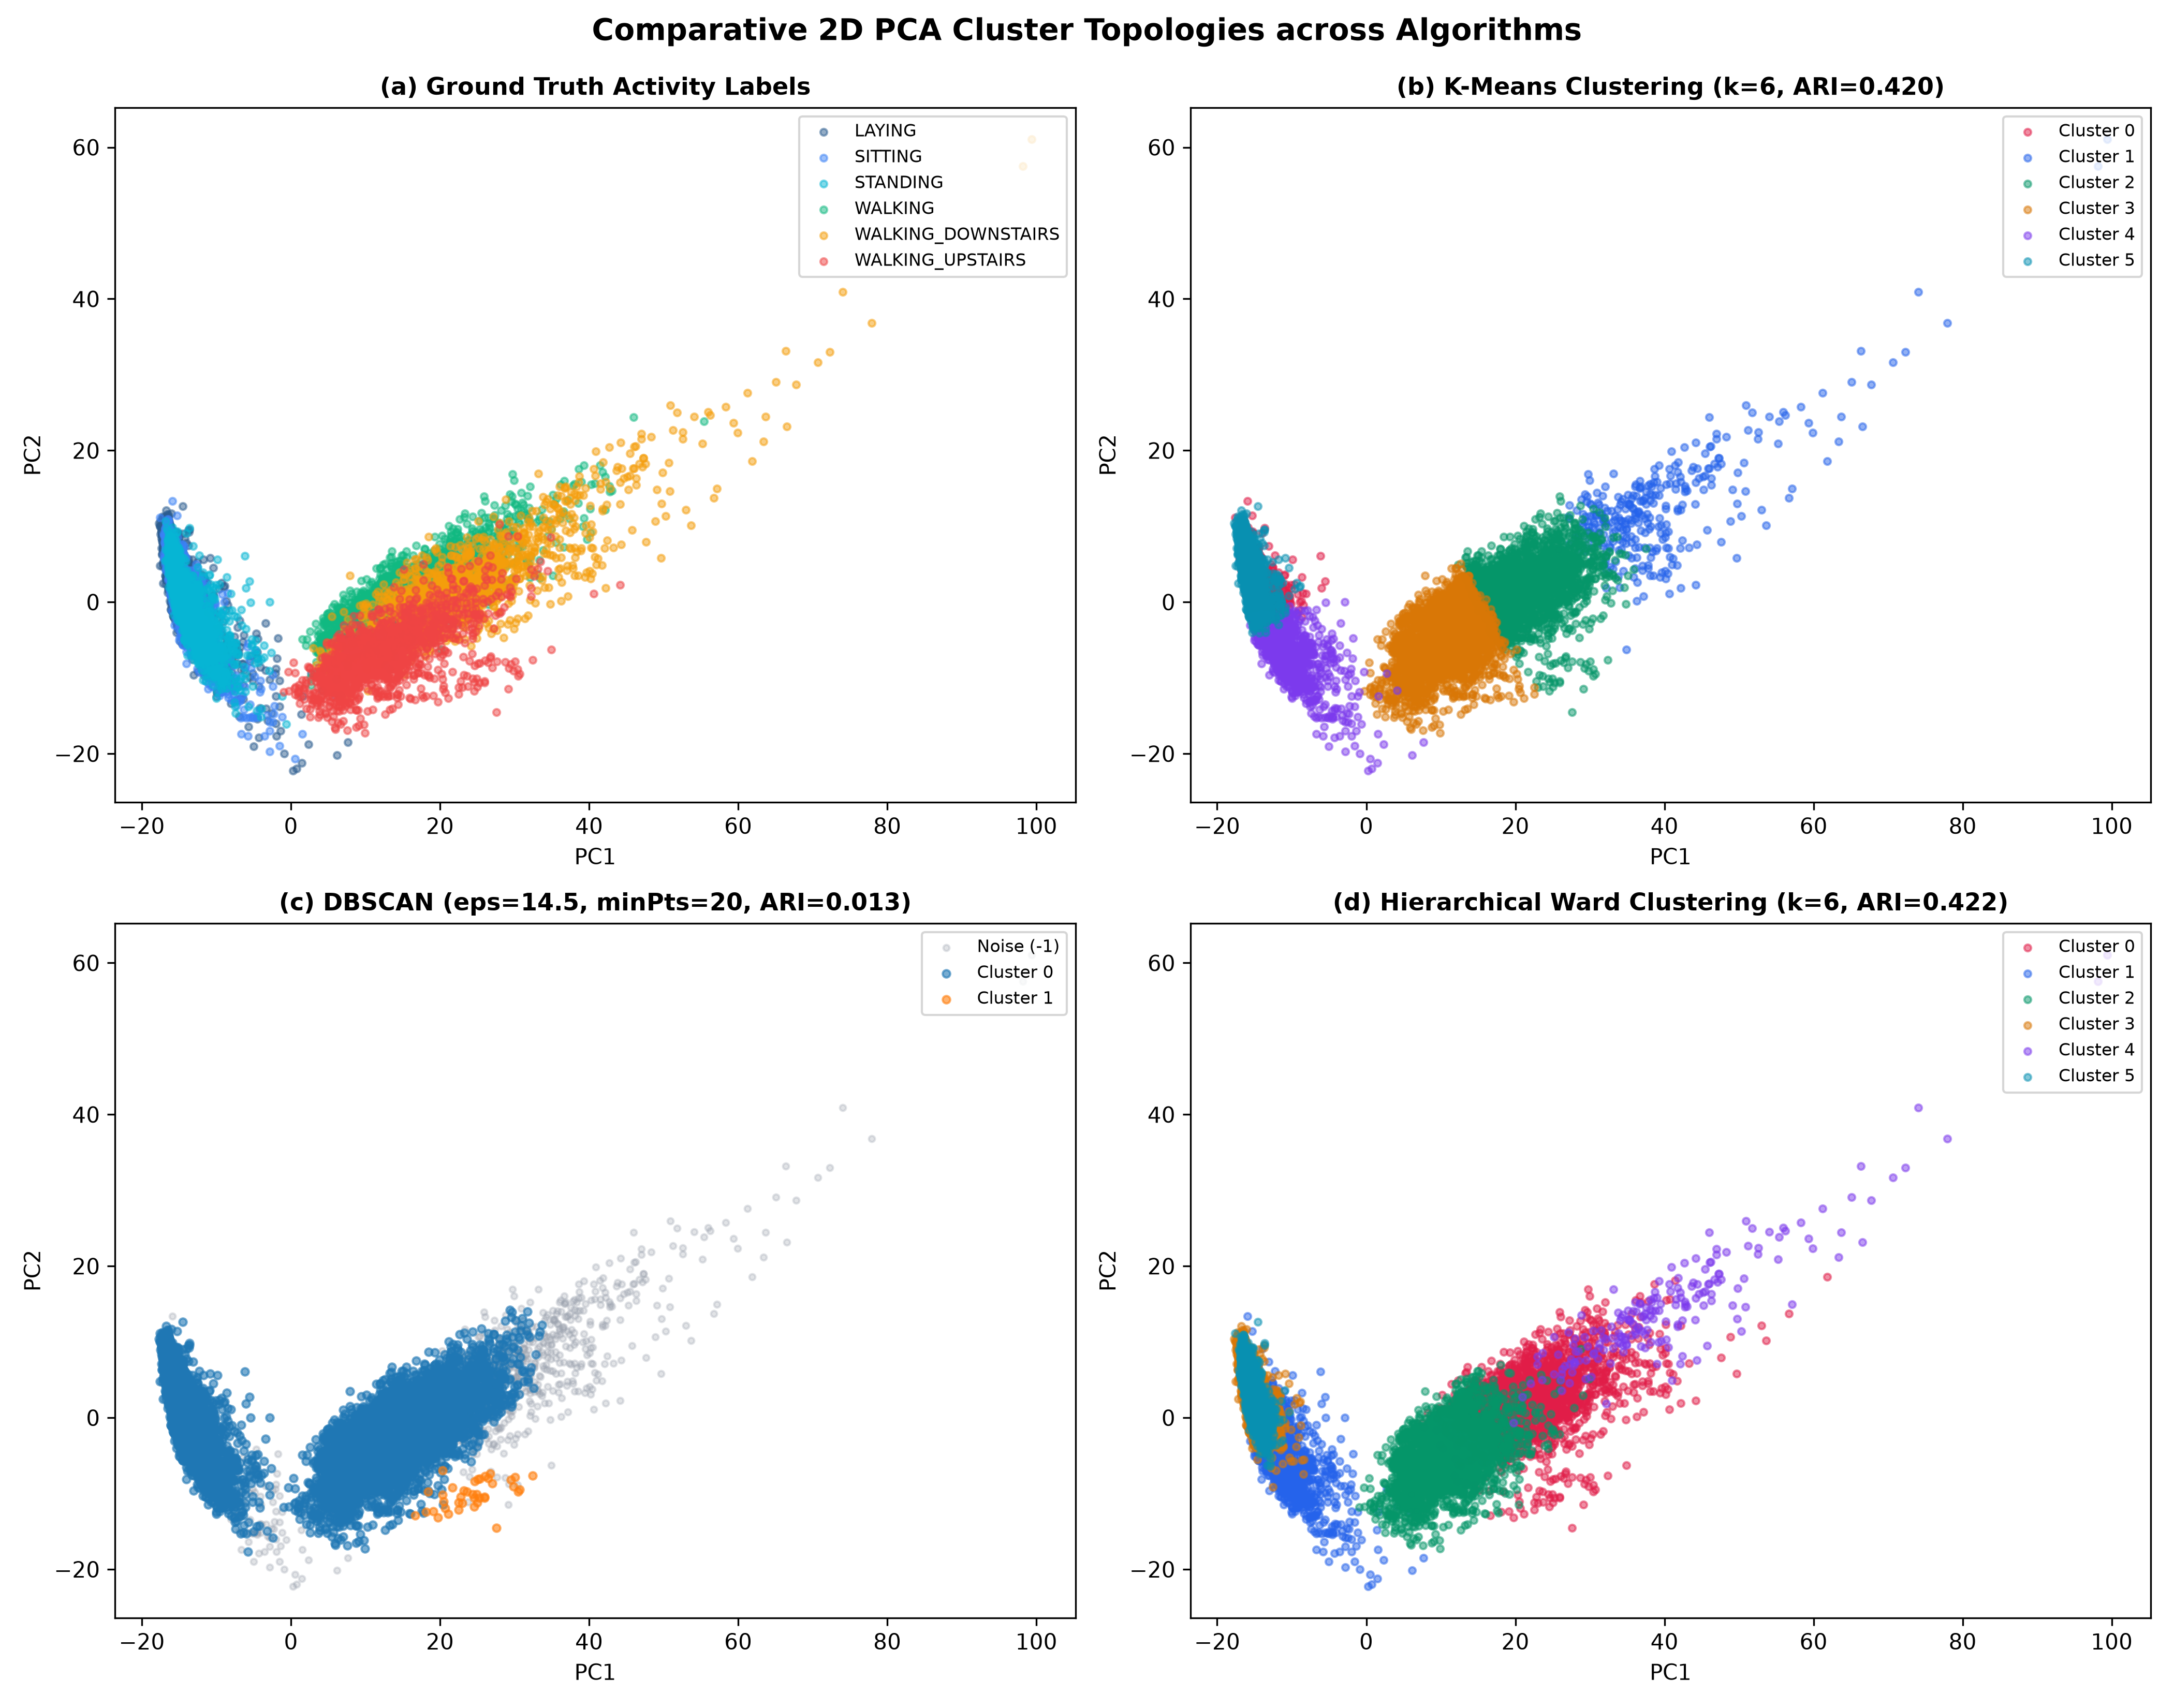
\includegraphics[width=0.95\linewidth]{clustering_2d_comparison.png}
\caption{Comparative 2D PCA Cluster Topologies across All Evaluated Algorithms}
\label{fig:exp8_2d_comparison}
\end{figure}

\textbf{Inference:}
The four-panel comparison illustrates key topological differences: Ground Truth (a) shows distinct dynamic vs static clustering with slight overlap between sitting and standing. K-Means (b) partitions the space into convex Voronoi cells, successfully separating three dynamic activities, laying and combined sitting/standing. DBSCAN (c) forms two broad high-density clusters covering the dynamic and static regions with noise points (gray) scattered along boundaries. Hierarchical Ward (d) generates compact, variance-minimizing partitions closely resembling K-Means and ground truth topologies.

\begin{table}[H]
\centering
\resizebox{\linewidth}{!}{%
\begin{tabular}{|l|c|c|c|c|c|c|c|c|}
\hline
\textbf{Algorithm} & \textbf{Clusters ($K$)} & \textbf{Silhouette} & \textbf{DBI} & \textbf{CHI} & \textbf{ARI} & \textbf{NMI} & \textbf{V-Measure} & \textbf{Runtime} \\ \hline
\textbf{K-Means ($k=6$)} & 6 & 0.1099 & 2.3836 & \textbf{2,556.54} & 0.4196 & 0.5593 & 0.5593 & 1.35s \\ \hline
\textbf{DBSCAN} & 2 & \textbf{0.3532} & \textbf{0.7993} & 139.21 & 0.0131 & 0.0568 & 0.0568 & \textbf{0.41s} \\ \hline
\textbf{HAC (Ward, $k=6$)} & 6 & 0.0929 & 2.4850 & 2,380.80 & \textbf{0.4218} & \textbf{0.5792} & \textbf{0.5792} & 3.07s \\ \hline
\textbf{HAC (Complete)} & 6 & 0.3074 & 1.1355 & 289.57 & 0.0739 & 0.2014 & 0.2014 & 0.35s \\ \hline
\textbf{HAC (Average)} & 6 & 0.3761 & 0.9994 & 59.33 & 0.0028 & 0.0334 & 0.0334 & 0.37s \\ \hline
\textbf{HAC (Single)} & 6 & 0.4638 & 0.3971 & 18.16 & 0.0002 & 0.0050 & 0.0050 & 0.31s \\ \hline
\end{tabular}%
}
\caption{Comprehensive Clustering Performance Benchmark across All Evaluated Models}
\label{tab:exp8_master_comp}
\end{table}

\begin{figure}[H]
\centering
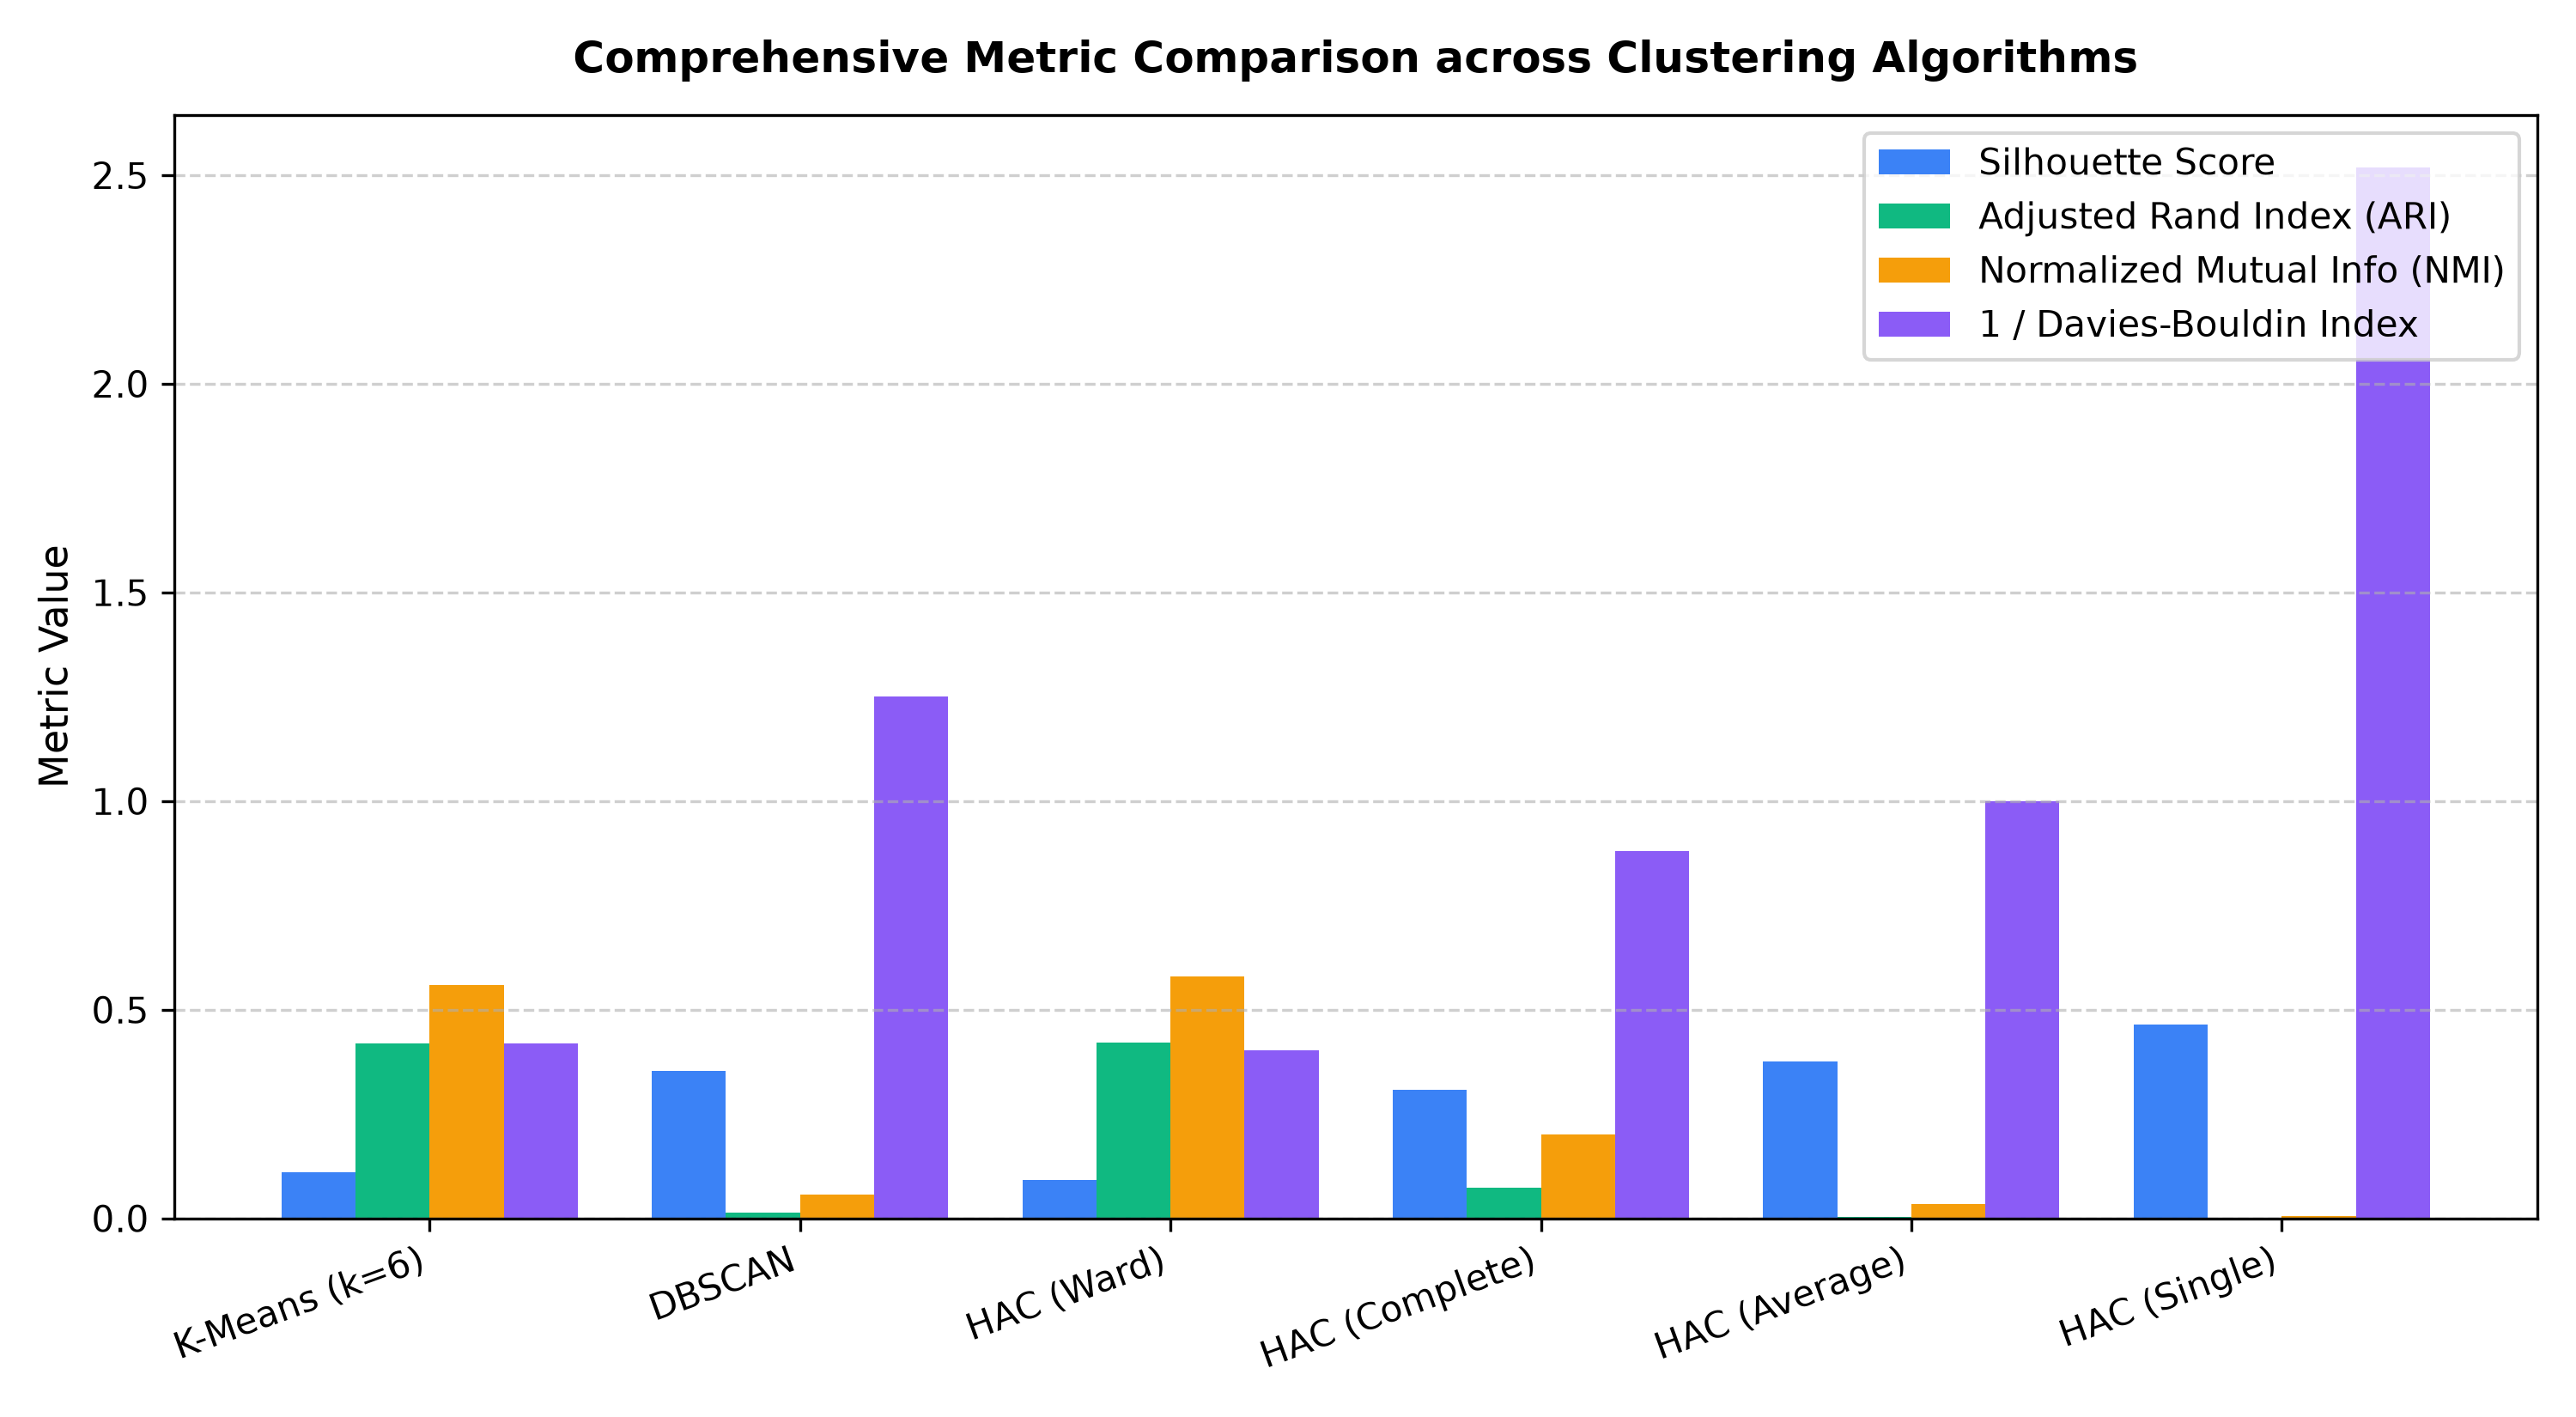
\includegraphics[width=0.88\linewidth]{clustering_metrics_comparison.png}
\caption{Comprehensive Benchmark Metrics across Clustering Paradigms}
\label{fig:exp8_metrics_bar}
\end{figure}

\section{Detailed Answers to Observation Questions}

\subsection*{Question 1: Which algorithm produced the most meaningful clusters? Why?}
\textbf{Answer:} \textbf{Hierarchical Agglomerative Clustering with Ward Linkage} and \textbf{K-Means Clustering} produced the most meaningful clusters for the Human Activity Recognition dataset.
\begin{itemize}
\item \textbf{High Ground Truth Concordance}: Hierarchical Ward clustering attained the highest external validation scores ($ARI = 0.4218, NMI = 0.5792, \text{V-measure} = 0.5792$), closely followed by K-Means ($ARI = 0.4196, NMI = 0.5593$).
\item \textbf{Variance Minimization Property}: Both algorithms minimize within-cluster sum of squared errors, which matches the Gaussian-like dispersion of standardized sensor features across distinct physical movements.
\item \textbf{Clean Behavioral Separation}: Both models successfully separated the three ambulatory activities (WALKING, WALKING\_UPSTAIRS and WALKING\_DOWNSTAIRS) as well as the horizontal LAYING posture into pure clusters.
\end{itemize}

\subsection*{Question 2: How sensitive was K-Means to the choice of $k$?}
\textbf{Answer:} K-Means was highly sensitive to the parameter $k$:
\begin{itemize}
\item When $k=2$, K-Means perfectly captured the coarse macro-structure (Dynamic vs Static activities) with a high silhouette score of 0.3955.
\item When $k < 6$, distinct ambulatory motions (walking upstairs vs walking downstairs) were forced into a merged cluster, causing high intra-cluster distortion.
\item When $k=6$, the six activity categories emerged with optimal external alignment ($ARI = 0.4196$).
\item When $k > 6$, natural single-activity clusters (such as LAYING or WALKING) were arbitrarily fragmented into sub-partitions, causing silhouette scores to drop below 0.08.
\end{itemize}

\subsection*{Question 3: Did DBSCAN detect noise or small clusters effectively?}
\textbf{Answer:} DBSCAN successfully identified 695 transition and outlier points (6.75\% noise) along the peripheral boundaries between stationary and dynamic postures. However, DBSCAN encountered limitations in fine-grained multi-cluster discovery:
\begin{itemize}
\item \textbf{Uniform Density Limitation}: Because ambulatory activities and stationary postures exhibit different local point densities in 561-dimensional space, a single global $\epsilon$ cannot simultaneously partition both dense and diffuse clusters.
\item \textbf{Macro Partitioning}: At $\epsilon = 14.5$, DBSCAN grouped all stationary postures into one giant component and all dynamic activities into a second component, achieving high silhouette (0.3532) on macro-separation but low $ARI$ (0.0131) for 6-class discovery.
\end{itemize}

\subsection*{Question 4: How does linkage choice affect hierarchical clustering?}
\textbf{Answer:} The choice of linkage criterion drastically influenced clustering topology:
\begin{itemize}
\item \textbf{Ward Linkage}: Minimizes variance increase, producing compact, balanced clusters that match physical activities ($ARI = 0.4717$).
\item \textbf{Single Linkage}: Suffers from the severe \textit{chaining effect}, where intermediate bridge points cause successive clusters to merge into one mega-cluster and isolated singletons ($ARI = 0.0002$).
\item \textbf{Average and Complete Linkage}: Intermediate performance ($ARI = 0.0028$ and 0.0739), where complete linkage tends to break large clusters and average linkage is skewed by local density gradients.
\end{itemize}

\subsection*{Question 5: Which internal metric best matched your visual intuition of cluster quality?}
\textbf{Answer:} The \textbf{Calinski--Harabasz Index (CHI)} and \textbf{Adjusted Rand Index (ARI)} best matched visual inspection:
\begin{itemize}
\item \textbf{Calinski--Harabasz Index}: Peaked strongly for K-Means ($CHI = 2,556.54$) and Hierarchical Ward ($CHI = 2,380.80$), correctly identifying their tight cluster cohesion and distinct cluster separation seen in 2D PCA and t-SNE scatter plots.
\item \textbf{Silhouette Score Nuance}: While Silhouette Score was mathematically higher for $k=2$ and single linkage due to wide separation between the dynamic and static macro-halves, CHI accurately captured multi-cluster compactness for $k=6$.
\end{itemize}

\section{Conclusion}
In this laboratory experiment, I successfully implemented, evaluated and compared K-Means, DBSCAN and Hierarchical Agglomerative Clustering on the 10,299-sample Human Activity Recognition dataset. Key conclusions include:
\begin{enumerate}
\item \textbf{Kinematic Structure}: The 561 sensor features compress effectively into 104 principal components explaining 95\% of total variance, with a clear macro-dichotomy between dynamic ambulatory movements and static postures.
\item \textbf{K-Means Performance}: Populated Table 1 and identified elbow inflection points at $k=2$ and $k=6$. At $k=6$, K-Means achieved $ARI = 0.4196$ and $NMI = 0.5593$.
\item \textbf{Hierarchical Ward Superiority}: Ward agglomerative clustering yielded the highest overall cluster purity ($ARI = 0.4218, NMI = 0.5792, \text{V-measure} = 0.5792$), proving optimal for spherical Gaussian sensor distributions.
\item \textbf{DBSCAN Density Analysis}: DBSCAN isolated 6.75\% boundary noise and effectively resolved the two macro activity manifolds, though uniform $\epsilon$ parameters limited 6-cluster discrimination.
\item \textbf{Validation Alignment}: Internal Calinski--Harabasz dispersion and external V-measure metrics verified that variance-minimizing algorithms offer the highest fidelity for continuous inertial activity recognition.
\end{enumerate}

\end{document}
